%%%%%%%%%%%%%%%%%%%%%%%%%%%%%%%%%%%%%%%%%
% Masters/Doctoral Thesis 
% LaTeX Template
% Version 2.5 (27/8/17)
%
% This template was downloaded from:
% http://www.LaTeXTemplates.com
%
% Version 2.x major modifications by:
% Vel (vel@latextemplates.com)
%
% This template is based on a template by:
% Steve Gunn (http://users.ecs.soton.ac.uk/srg/softwaretools/document/templates/)
% Sunil Patel (http://www.sunilpatel.co.uk/thesis-template/)
%
% Template license:
% CC BY-NC-SA 3.0 (http://creativecommons.org/licenses/by-nc-sa/3.0/)
%
%%%%%%%%%%%%%%%%%%%%%%%%%%%%%%%%%%%%%%%%%

%----------------------------------------------------------------------------------------
%	PACKAGES AND OTHER DOCUMENT CONFIGURATIONS
%----------------------------------------------------------------------------------------

\documentclass[
11pt, % The default document font size, options: 10pt, 11pt, 12pt
%oneside, % Two side (alternating margins) for binding by default, uncomment to switch to one side
greek,english,% ngerman for German
singlespacing, % Single line spacing, alternatives: onehalfspacing or doublespacing
%draft, % Uncomment to enable draft mode (no pictures, no links, overfull hboxes indicated)
%nolistspacing, % If the document is onehalfspacing or doublespacing, uncomment this to set spacing in lists to single
%liststotoc, % Uncomment to add the list of figures/tables/etc to the table of contents
%toctotoc, % Uncomment to add the main table of contents to the table of contents
%parskip, % Uncomment to add space between paragraphs
%nohyperref, % Uncomment to not load the hyperref package
headsepline, % Uncomment to get a line under the header
%chapterinoneline, % Uncomment to place the chapter title next to the number on one line
%consistentlayout, % Uncomment to change the layout of the declaration, abstract and acknowledgements pages to match the default layout
]{MastersDoctoralThesis} % The class file specifying the document structure


\usepackage[utf8]{inputenc} % Required for inputting international characters

\usepackage[LSF,LGR,T3,T1]{fontenc} % Output font encoding for international characters
\emergencystretch=1em

\usepackage{mathpazo} % Use the Palatino font by default

\usepackage[backend=biber,style=numeric,citestyle=numeric,natbib=true]{biblatex} % Use the bibtex backend with the authoryear citation style (which resembles APA)

\addbibresource{references_new.bib} % The filename of the bibliography

\usepackage[autostyle=true]{csquotes} % Required to generate language-dependent quotes in the bibliography

\usepackage{float}

\usepackage{array,multirow}
\usepackage[stretch=10,shrink=10]{microtype}

\usepackage{amsmath}

\usepackage{subfig}

\usepackage{comment}


\newcaptionname{greek}{\facname}{}
\newcaptionname{greek}{\univname}{Εθνικό και Καποδιστριακό Πανεπιστήμιο Αθηνών}
\newcaptionname{greek}{\degreename}{}
\newcaptionname{greek}{\deptname}{}
\newcaptionname{greek}{\authorname}{Παναγιώτη Μητσόπουλο}
%\newcaptionname{greek}{\byname}{του}


%----------------------------------------------------------------------------------------
%	MARGIN SETTINGS
%----------------------------------------------------------------------------------------

\geometry{
	paper=a4paper, % Change to letterpaper for US letter
	inner=2.5cm, % Inner margin
	outer=2.5cm, % Outer margin
	bindingoffset=.5cm, % Binding offset
	top=1.5cm, % Top margin
	bottom=1.5cm, % Bottom margin
	%showframe, % Uncomment to show how the type block is set on the page
}

%----------------------------------------------------------------------------------------
%	THESIS INFORMATION
%----------------------------------------------------------------------------------------

\thesistitle{Estimation and mechanistic interpretation of wind-wave interactions in \emph{in situ} and satellite altimetry data in the Southern New England Region.} % Your thesis title, this is used in the title and abstract, print it elsewhere with \ttitle
\supervisor{Sarantis Sofianos} % Your supervisor's name, this is used in the title page, print it elsewhere with \supname
\examiner{Helena Floca} % Your examiner's name, this is not currently used anywhere in the template, print it elsewhere with \examname
\degree{Master of Science} % Your degree name, this is used in the title page and abstract, print it elsewhere with \degreename
\author{Panagiotis Mitsopoulos} % Your name, this is used in the title page and abstract, print it elsewhere with \authorname
\addresses{} % Your address, this is not currently used anywhere in the template, print it elsewhere with \addressname

\subject{Physical Oceanography} % Your subject area, this is not currently used anywhere in the template, print it elsewhere with \subjectname
\keywords{} % Keywords for your thesis, this is not currently used anywhere in the template, print it elsewhere with \keywordnames
\university{\href{https://en.uoa.gr/}{National and Kapodistrian University of Athens}} % Your university's name and URL, this is used in the title page and abstract, print it elsewhere with \univname
\department{\href{https://oceanography.geol.uoa.gr/}{Oceanography and Management of the Marine Environment MSc}} % Your department's name and URL, this is used in the title page and abstract, print it elsewhere with \deptname
\group{\href{http://www.oc.phys.uoa.gr/index.html}{Ocean Physics And Modelling Group}} % Your research group's name and URL, this is used in the title page, print it elsewhere with \groupname
\faculty{\href{}{Sarantis Sofianos}} % Your faculty's name and URL, this is used in the title page and abstract, print it elsewhere with \facname

\AtBeginDocument{
\hypersetup{pdftitle=\ttitle} % Set the PDF's title to your title
\hypersetup{pdfauthor=\authorname} % Set the PDF's author to your name
\hypersetup{pdfkeywords=\keywordnames} % Set the PDF's keywords to your keywords
}


\begin{document}

\frontmatter % Use roman page numbering style (i, ii, iii, iv...) for the pre-content pages

\pagestyle{plain} % Default to the plain heading style until the thesis style is called for the body content

%----------------------------------------------------------------------------------------
%	TITLE PAGE
%----------------------------------------------------------------------------------------

\begin{titlepage}
\begin{center}

\vspace*{.06\textheight}
{\scshape\LARGE \univname\par}\vspace{1.5cm} % University name
\textsc{\Large Master's Thesis}\\[0.5cm] % Thesis type

\HRule \\[0.4cm] % Horizontal line
{\huge \bfseries \ttitle\par}\vspace{0.4cm} % Thesis title
\HRule \\[1.5cm] % Horizontal line
 
\begin{minipage}[t]{0.4\textwidth}
\begin{flushleft} \large
\emph{Author:}\\
\href{https://www.researchgate.net/profile/Panagiotis_Mitsopoulos2}{\authorname} % Author name - remove the \href bracket to remove the link
\end{flushleft}
\end{minipage}
\begin{minipage}[t]{0.4\textwidth}
\begin{flushright} \large
\emph{Supervisor:} \\
\href{}{\supname} % Supervisor name - remove the \href bracket to remove the link 

\emph{Advisory Committe:}\\
\href{}{\examname},
\href{https://cee.engr.uconn.edu/people/pena-malaquias}{Malaquias Peña}
\end{flushright}
\end{minipage}\\[3cm]
 
\vfill

\large \textit{A thesis submitted in fulfillment of the requirements\\ for the degree of \degreename}\\[0.3cm] % University requirement text
\textit{in the}\\[0.4cm]
\deptname\\\groupname\\[2cm] % Research group name and department name
 
\vfill

{\large \today}\\[4cm] % Date
%\includegraphics{Logo} % University/department logo - uncomment to place it
 
\vfill
\end{center}
\end{titlepage}

%----------------------------------------------------------------------------------------
%	DECLARATION PAGE
%----------------------------------------------------------------------------------------

\begin{declaration}
\addchaptertocentry{\authorshipname} % Add the declaration to the table of contents
\noindent I, \authorname, declare that this thesis titled, \enquote{\ttitle} and the work presented in it are my own. I confirm that:

\begin{itemize} 
\item This work was done wholly or mainly while in candidature for a research degree at this University.
\item Where any part of this thesis has previously been submitted for a degree or any other qualification at this University or any other institution, this has been clearly stated.
\item Where I have consulted the published work of others, this is always clearly attributed.
\item Where I have quoted from the work of others, the source is always given. With the exception of such quotations, this thesis is entirely my own work.
\item I have acknowledged all main sources of help.
\item Where the thesis is based on work done by myself jointly with others, I have made clear exactly what was done by others and what I have contributed myself.
\end{itemize}
 
\noindent Signed:\\
\rule[0.5em]{25em}{0.5pt} % This prints a line for the signature
 
\noindent Date:\\
\rule[0.5em]{25em}{0.5pt} % This prints a line to write the date
\end{declaration}

\cleardoublepage


%----------------------------------------------------------------------------------------
%	QUOTATION PAGE
%----------------------------------------------------------------------------------------

\begin{comment}


\vspace*{0.2\textheight}

\noindent\enquote{\itshape Thanks to my solid academic training, today I can write hundreds of words on virtually any topic without possessing a shred of information, which is how I got a good job in journalism.}\bigbreak

\hfill Dave Barry

\end{comment}


%----------------------------------------------------------------------------------------
%	ABSTRACT PAGE
%----------------------------------------------------------------------------------------

\begin{abstract}
\addchaptertocentry{\abstractname} % Add the abstract to the table of contents

Accurate estimation of wind and wave conditions is an essential information resource for ship routing, coastal engineering, and several other coastal activities. The developing offshore wind energy industry needs these estimations for prospecting and ensuring the optimal siting of wind farms. Wind farms' construction, operation, and decommission need real-time monitoring of wind and waves for decision making. Additionally, special attention to extremes and transient events must be paid for the aforementioned applications since they have the most considerable impact and must be well captured in numerical models. While a sprawl of data from various remote sensing capabilities, including the next generation of satellite altimeter data, is growing, their use is more effective when combined with traditional, longer-record, in situ observations from buoys, which serve as ground truth reference. This study focuses on the independent use  of the two data sources and properly combining them so that the final analysis is physically consistent. Statistical analysis and kriging interpolation merging multiple sensor’s data are performed to improve the offshore marine conditions' estimations and to identify dominant mesoscale and local mechanisms that contribute to their variability. The scope of this research is focused on the observations taken on the Southern New England region in the United States, where new offshore wind energy developments are taking place.

\vspace{6mm}

\emph{Main research results:}
\begin{itemize}
  \item An updated wind and wave climatology of the domain with a focus on climate variability in multiple timescales (diurnal, seasonal, interannual).
  \item The directional distribution of near-surface wind and wave height.
  \item The wind speed and significant wave height relationship based on theoretical formulae and ocean waves classification based on their growth rate.
  \item The wind speed probability density functions which provide the best fit to the wind speed distribution.
  \item A case study of extreme events.
  \item The validation of satellite altimeter with in situ observations in the Southern New England region.
  \item Maps of interpolated wind speed and significant wave height fields using observations from multiple satellite altimeters.
\end{itemize}

\end{abstract}


\newcaptionname{greek}{\thesistitle}{Εκτίμηση και ερμηνεία των φυσικών μηχανισμών αλληλεπίδρασης θάλασσας-ατμόσφαιρας, μέσω δεδομένων ανέμου και ύψους κύματος, από πλωτούς σταθμούς μέτρησης και δορυφόρους νέας γενιάς στην περιοχή της Νότιας Νέας Αγγλίας.}

{\selectlanguage{greek}

\begin{abstract}
%\addchaptertocentry{\abstractname} % Add the abstract to the table of contents

Η ακριβής εκτίμηση των συνθηκών ανέμου και κύματος αποτελεί απαραίτητη πληροφορία για την πορεία των πλοίων, την παράκτια μηχανική και πολλών ακόμη δραστηριοτήτων που λαμβάνουν χώρα στη παράκτια ζώνη. Η αναπτυσσόμενη βιομηχανία της υπεράκτιας αιολικής ενέργειας χρειάζεται αυτές τις εκτιμήσεις για την έρευνα και εξασφάλιση της βέλτιστης τοποθεσίας για τα αιολικά πάρκα. Η παρακολούθηση σε πραγματικό χρόνο του ανέμου και του κύματος για την λήψη αποφάσεων είναι απαραίτητη κατά τις περιόδους κατασκευής, λειτουργίας αλλά και απόσυρσης των αιολικών πάρκων. Επιπροσθέτως, ιδιαίτερη σημασία πρέπει να δίδεται και στα ακραία και παροδικά φαινόμενα καθώς έχουν τις σημαντικότερες επιπτώσεις και πρέπει να αποτυπώνονται ρεαλιστικά από τα αριθμητικά μοντέλα. Καθώς η διαθεσιμότητα των δεδομένων τηλεπισκόπισης, συμπεριλαμβανωμένων και των δορυφόρων αλτιμετρίας νέας γενιάς, ολοένα και αναπτύσσεται, η χρήση τους είναι πιο αποτελεσματική όταν συνδυάζεται με επιτόπιες παρατηρήσεις από τους πιο παραδοσιακούς, πλωτούς σταθμούς μέτρησης, οι οποίοι συλλέγουν δεδομένα για μεγάλο χρονικό διάστημα και θεωρούνται ως παρατηρήσεις αναφοράς. Η συγκεκριμένη εργασία εστιάζεται στην ανεξάρτητη ανάλυση των δύο πηγών δεδομένων αλλά και στον κατάλληλο συνδυασμό τους ώστε τα τελικά αποτελέσματα να εμφανίζουν συνέπεια. Η στατιστική ανάλυση επιτόπιων παρατηρήσεων αλλά και η εφαρμογή σχήματος παρεμβολής με την αριθμητική μέθοδο \selectlanguage{english}kriging\selectlanguage{greek} για την συγχώνευση δεδομένων από διαφορετικούς δορυφόρους, βοηθούν στην βελτίωση της εκτίμησης των υπεράκτιων θαλάσσιων συνθηκών αλλά και στην αναγνώριση των κυρίαρχων τοπικών μηχανισμών και μέσης κλίμακας που συμβάλλουν στην μεταβλητότητα τους. Η περιοχή μελέτης είναι η ακτή της Νότιας Νέας Αγγλίας των Ηνωμένων Πολιτειών της Αμερικής, στην οποία λαμβάνει χώρα η ανάπτυξη της υπεράκτιας αιολικής ενέργειας.
\begin{comment}


\vspace{4mm}

\emph{Main research results:}
\begin{itemize}
  \item An updated wind and wave climatology of the domain with a focus on climate variability in multiple timescales (diurnal, seasonal, interannual).
  \item The directional distribution of near-surface wind and wave height.
  \item The wind speed and significant wave height relationship based on theoretical formulae and ocean waves classification based on their growth rate.
  \item The wind speed probability density functions which provide the best fit to the wind speed distribution.
  \item A case study of extreme events.
  \item The validation of satellite altimeter with in situ observations in the Southern New England region.
  \item Maps of interpolated wind speed and significant wave height fields using observations from multiple satellite altimeters.
\end{itemize}
\end{comment}

\end{abstract}
}

\selectlanguage{english}

%-----------------------------------------------------------------------
----------------


\begin{comment}
%\selectlanguage{greek}
%\begin{otherlanguage*}{greek}
\begin{titlepage}
\begin{center}
   Περίληη
\end{center}


\textgreek{Περίληψη} 
Per'ilhqh
\vspace{6mm}

\emph{φγ}
\begin{itemize}
  \item γσργ.

\end{itemize}


\end{titlepage}

\end{comment}
%\selectlanguage{english}
%\end{otherlanguage*}



%---------------------------------------------------------------------------



%----------------------------------------------------------------------------------------
%	ACKNOWLEDGEMENTS
%----------------------------------------------------------------------------------------

\begin{acknowledgements}
\addchaptertocentry{\acknowledgementname} % Add the acknowledgements to the table of contents
Looking back at the year that I spent working on my thesis, I would like to thank the people who contributed to its realization, both academically and personally.

First and foremost, my deepest gratitude goes to my supervisor, Professor Sarantis Sofianos, to support my willingness to work on this thesis and his guidance, encouragement, and thoughtful comments.

I would also like to express my great appreciation to Professor Malaquias  Peña. His experience and expertise were critical from the foundation of this thesis to its completion. It was a pleasure to collaborate and share my ideas with him during the past year.

My sincere appreciation goes to Professor Helena Floca. She was always present and helpful when I needed her support as a member of the advisory committee and one of the Oceanography and Management of the Marine Environment faculty members.

I cannot omit to thank John Karagiorgos and all members of the Ocean Physics and Modelling Group, of which I spent one memorable year as a member. They provided me with insight into technical matters, were there to discuss, encouraged me, and assisted me as a friend and colleague. 

I am also thankful to Randolph Bucciarelli and the CDIP research team for their cooperation and effort to provide me with valuable information and data. Stylianos Flampouris of NOAA-NCEP-EMC was kind enough to share his ocean waves' expertise and correspond to my inquiries.

On a personal level, I would like to express my gratitude to my parents for their support and belief in my aspirations. Last but not least, a heartfelt thank you goes to Viky K.  for her patience, understanding and sharing a challenging but rewarding year.
\end{acknowledgements}

%----------------------------------------------------------------------------------------
%	LIST OF CONTENTS/FIGURES/TABLES PAGES
%----------------------------------------------------------------------------------------

\tableofcontents % Prints the main table of contents

\listoffigures % Prints the list of figures

\listoftables % Prints the list of tables

%----------------------------------------------------------------------------------------
%	ABBREVIATIONS
%----------------------------------------------------------------------------------------

\begin{abbreviations}{ll} % Include a list of abbreviations (a table of two columns)

\textbf{SWH} & \textbf{S}ignificant \textbf{W}ave \textbf{H}eight\\
\textbf{WS} & \textbf{W}ind \textbf{S}peed\\
\textbf{SSH} & \textbf{S}ea \textbf{S}urface \textbf{H}eight\\
\textbf{SST} & \textbf{S}ea \textbf{S}urface \textbf{T}emperature\\
\textbf{SNE} & \textbf{S}outhern \textbf{N}ew \textbf{E}ngland\\
\textbf{NDBC} & \textbf{N}ational \textbf{D}ata \textbf{B}uoy \textbf{C}enter\\
\textbf{CDIP} & \textbf{C}oastal \textbf{D}ata \textbf{I}nformation \textbf{P}rogram\\
\textbf{OERG} & \textbf{O}cean \textbf{E}ngineering \textbf{R}esearch \textbf{G}roup\\
\textbf{IOD} & \textbf{I}ntegrative \textbf{O}ceanography \textbf{D}ivision\\
\textbf{SIO} & \textbf{S}cripps \textbf{I}nstitution of \textbf{O}ceanography\\
\textbf{LISICOS} & \textbf{L}ong \textbf{I}sland \textbf{S}ound \textbf{I}ntegrated \textbf{C}oastal \textbf{O}bserving \textbf{S}ystem\\
\textbf{UConn} & \textbf{U}niversity of \textbf{Conn}ecticut\\
\textbf{NOAA} & \textbf{N}ational \textbf{O}ceanic and \textbf{A}tmospheric \textbf{A}dministration\\
\textbf{THREDDS} & \textbf{TH}ematic \textbf{R}eal-time \textbf{E}nvironmental \textbf{D}istributed \textbf{D}ata \textbf{S}ervices\\
\textbf{TDS} & \textbf{T}hredds \textbf{D}ata \textbf{S}erver\\
\textbf{NetCDF} & \textbf{Net}work \textbf{C}ommon \textbf{D}ata \textbf{F}orm\\
\textbf{BOEM} & \textbf{B}ureau of \textbf{O}cean \textbf{E}nergy \textbf{M}anagement\\
\textbf{CNES} & \textbf{C}entre \textbf{N}ational d'\textbf{E}tudes \textbf{S}patiales\\
\textbf{ISRO} & \textbf{I}ndian \textbf{S}pace and \textbf{R}esearch \textbf{O}rganization\\
\textbf{NASA} & \textbf{N}ational \textbf{A}eronautics and \textbf{S}pace \textbf{A}dministration\\
\textbf{EUMETSAT} & \textbf{EU}ropean Organization for the exploitation of \textbf{MET}eorological \textbf{SAT}ellites\\
\textbf{ESA} & \textbf{E}uropean \textbf{S}pace \textbf{A}gency\\
\textbf{LRM} & \textbf{L}ow \textbf{R}esolution \textbf{M}ode\\
\textbf{PLRM} & \textbf{Pseudo} \textbf{L}ow \textbf{R}esolution \textbf{M}ode\\
\textbf{SAR} & \textbf{S}ynthetic \textbf{A}perture \textbf{R}adar\\
\textbf{SARIn} & \textbf{S}ynthetic \textbf{A}perture \textbf{R}adar \textbf{Interferometry}\\
\textbf{AMR} & \textbf{A}dvanced \textbf{M}icrowave \textbf{R}adiometer\\
\textbf{LRA} & \textbf{L}aser \textbf{R}eflector \textbf{A}rray\\
\textbf{GPSP} & \textbf{G}lobal \textbf{P}ositioning \textbf{S}ystem \textbf{P}ayload\\
\textbf{NRT} & \textbf{N}ear \textbf{R}eal \textbf{T}ime\\
\textbf{GDR} & \textbf{G}eophysical \textbf{D}ata \textbf{R}ecords\\
\textbf{OGDR} & \textbf{O}perational \textbf{G}eophysical \textbf{D}ata \textbf{R}ecords\\
\textbf{IGDR} & \textbf{I}nterim \textbf{G}eophysical \textbf{D}ata \textbf{R}ecords\\
\textbf{STC} & \textbf{S}hort \textbf{T}ime \textbf{C}ritical\\
\textbf{NTC} & \textbf{N}on \textbf{T}ime \textbf{C}ritical\\
\textbf{GOP} & \textbf{G}eophysical \textbf{O}cean \textbf{P}roduct\\
\textbf{CUT} & \textbf{C}ryosat \textbf{U}ser \textbf{T}ool\\
\textbf{WPC} & \textbf{W}eather \textbf{P}rediction \textbf{C}enter\\


\end{abbreviations}

%----------------------------------------------------------------------------------------
%	PHYSICAL CONSTANTS/OTHER DEFINITIONS
%----------------------------------------------------------------------------------------
\begin{comment}

\begin{constants}{lr@{${}={}$}l} % The list of physical constants is a three column table

% The \SI{}{} command is provided by the siunitx package, see its documentation for instructions on how to use it

Speed of Light & $c_{0}$ & \SI{2.99792458e8}{\meter\per\second} (exact)\\
%Constant Name & $Symbol$ & $Constant Value$ with units\\

\end{constants}

\end{comment}

%----------------------------------------------------------------------------------------
%	SYMBOLS
%----------------------------------------------------------------------------------------


\begin{comment}
\begin{symbols}{lll} % Include a list of Symbols (a three column table)

$a$ & distance & \si{\meter} \\
$P$ & power & \si{\watt} (\si{\joule\per\second}) \\
%Symbol & Name & Unit \\

\addlinespace % Gap to separate the Roman symbols from the Greek

$\omega$ & angular frequency & \si{\radian} \\

\end{symbols}
\end{comment}


%----------------------------------------------------------------------------------------
%	DEDICATION
%----------------------------------------------------------------------------------------


\begin{comment}

\dedicatory{For/Dedicated to/To my\ldots} 

\end{comment}


%----------------------------------------------------------------------------------------
%	THESIS CONTENT - CHAPTERS
%----------------------------------------------------------------------------------------

\mainmatter % Begin numeric (1,2,3...) page numbering

\pagestyle{thesis} % Return the page headers back to the "thesis" style

% Include the chapters of the thesis as separate files from the Chapters folder
% Uncomment the lines as you write the chapters

% Chapter 1

\chapter{Introduction} % Main chapter title

\label{Chapter1} % For referencing the chapter elsewhere, use \ref{Chapter1} 

%----------------------------------------------------------------------------------------

% Define some commands to keep the formatting separated from the content 
\newcommand{\keyword}[1]{\textbf{#1}}
\newcommand{\tabhead}[1]{\textbf{#1}}
\newcommand{\code}[1]{\texttt{#1}}
\newcommand{\file}[1]{\texttt{\bfseries#1}}
\newcommand{\option}[1]{\texttt{\itshape#1}}

%----------------------------------------------------------------------------------------

\section{Welcome and Thank You}
Welcome to this \LaTeX{} Thesis Template, a beautiful and easy to use template for writing a thesis using the \LaTeX{} typesetting system.

If you are writing a thesis (or will be in the future) and its subject is technical or mathematical (though it doesn't have to be), then creating it in \LaTeX{} is highly recommended as a way to make sure you can just get down to the essential writing without having to worry over formatting or wasting time arguing with your word processor.

\LaTeX{} is easily able to professionally typeset documents that run to hundreds or thousands of pages long. With simple mark-up commands, it automatically sets out the table of contents, margins, page headers and footers and keeps the formatting consistent and beautiful. One of its main strengths is the way it can easily typeset mathematics, even \emph{heavy} mathematics. Even if those equations are the most horribly twisted and most difficult mathematical problems that can only be solved on a super-computer, you can at least count on \LaTeX{} to make them look stunning.

%----------------------------------------------------------------------------------------

\section{Learning \LaTeX{}}

\LaTeX{} is not a \textsc{wysiwyg} (What You See is What You Get) program, unlike word processors such as Microsoft Word or Apple's Pages. Instead, a document written for \LaTeX{} is actually a simple, plain text file that contains \emph{no formatting}. You tell \LaTeX{} how you want the formatting in the finished document by writing in simple commands amongst the text, for example, if I want to use \emph{italic text for emphasis}, I write the \verb|\emph{text}| command and put the text I want in italics in between the curly braces. This means that \LaTeX{} is a \enquote{mark-up} language, very much like HTML.

\subsection{A (not so short) Introduction to \LaTeX{}}

If you are new to \LaTeX{}, there is a very good eBook -- freely available online as a PDF file -- called, \enquote{The Not So Short Introduction to \LaTeX{}}. The book's title is typically shortened to just \emph{lshort}. You can download the latest version (as it is occasionally updated) from here:
\url{http://www.ctan.org/tex-archive/info/lshort/english/lshort.pdf}

It is also available in several other languages. Find yours from the list on this page: \url{http://www.ctan.org/tex-archive/info/lshort/}

It is recommended to take a little time out to learn how to use \LaTeX{} by creating several, small `test' documents, or having a close look at several templates on:\\ 
\url{http://www.LaTeXTemplates.com}\\ 
Making the effort now means you're not stuck learning the system when what you \emph{really} need to be doing is writing your thesis.

\subsection{A Short Math Guide for \LaTeX{}}

If you are writing a technical or mathematical thesis, then you may want to read the document by the AMS (American Mathematical Society) called, \enquote{A Short Math Guide for \LaTeX{}}. It can be found online here:
\url{http://www.ams.org/tex/amslatex.html}
under the \enquote{Additional Documentation} section towards the bottom of the page.

\subsection{Common \LaTeX{} Math Symbols}
There are a multitude of mathematical symbols available for \LaTeX{} and it would take a great effort to learn the commands for them all. The most common ones you are likely to use are shown on this page:
\url{http://www.sunilpatel.co.uk/latex-type/latex-math-symbols/}

You can use this page as a reference or crib sheet, the symbols are rendered as large, high quality images so you can quickly find the \LaTeX{} command for the symbol you need.

\subsection{\LaTeX{} on a Mac}
 
The \LaTeX{} distribution is available for many systems including Windows, Linux and Mac OS X. The package for OS X is called MacTeX and it contains all the applications you need -- bundled together and pre-customized -- for a fully working \LaTeX{} environment and work flow.
 
MacTeX includes a custom dedicated \LaTeX{} editor called TeXShop for writing your `\file{.tex}' files and BibDesk: a program to manage your references and create your bibliography section just as easily as managing songs and creating playlists in iTunes.

%----------------------------------------------------------------------------------------

\section{Getting Started with this Template}

If you are familiar with \LaTeX{}, then you should explore the directory structure of the template and then proceed to place your own information into the \emph{THESIS INFORMATION} block of the \file{main.tex} file. You can then modify the rest of this file to your unique specifications based on your degree/university. Section \ref{FillingFile} on page \pageref{FillingFile} will help you do this. Make sure you also read section \ref{ThesisConventions} about thesis conventions to get the most out of this template.

If you are new to \LaTeX{} it is recommended that you carry on reading through the rest of the information in this document.

Before you begin using this template you should ensure that its style complies with the thesis style guidelines imposed by your institution. In most cases this template style and layout will be suitable. If it is not, it may only require a small change to bring the template in line with your institution's recommendations. These modifications will need to be done on the \file{MastersDoctoralThesis.cls} file.

\subsection{About this Template}

This \LaTeX{} Thesis Template is originally based and created around a \LaTeX{} style file created by Steve R.\ Gunn from the University of Southampton (UK), department of Electronics and Computer Science. You can find his original thesis style file at his site, here:
\url{http://www.ecs.soton.ac.uk/~srg/softwaretools/document/templates/}

Steve's \file{ecsthesis.cls} was then taken by Sunil Patel who modified it by creating a skeleton framework and folder structure to place the thesis files in. The resulting template can be found on Sunil's site here:
\url{http://www.sunilpatel.co.uk/thesis-template}

Sunil's template was made available through \url{http://www.LaTeXTemplates.com} where it was modified many times based on user requests and questions. Version 2.0 and onwards of this template represents a major modification to Sunil's template and is, in fact, hardly recognisable. The work to make version 2.0 possible was carried out by \href{mailto:vel@latextemplates.com}{Vel} and Johannes Böttcher.

%----------------------------------------------------------------------------------------

\section{What this Template Includes}

\subsection{Folders}

This template comes as a single zip file that expands out to several files and folders. The folder names are mostly self-explanatory:

\keyword{Appendices} -- this is the folder where you put the appendices. Each appendix should go into its own separate \file{.tex} file. An example and template are included in the directory.

\keyword{Chapters} -- this is the folder where you put the thesis chapters. A thesis usually has about six chapters, though there is no hard rule on this. Each chapter should go in its own separate \file{.tex} file and they can be split as:
\begin{itemize}
\item Chapter 1: Introduction to the thesis topic
\item Chapter 2: Background information and theory
\item Chapter 3: (Laboratory) experimental setup
\item Chapter 4: Details of experiment 1
\item Chapter 5: Details of experiment 2
\item Chapter 6: Discussion of the experimental results
\item Chapter 7: Conclusion and future directions
\end{itemize}
This chapter layout is specialised for the experimental sciences, your discipline may be different.

\keyword{Figures} -- this folder contains all figures for the thesis. These are the final images that will go into the thesis document.

\subsection{Files}

Included are also several files, most of them are plain text and you can see their contents in a text editor. After initial compilation, you will see that more auxiliary files are created by \LaTeX{} or BibTeX and which you don't need to delete or worry about:

\keyword{example.bib} -- this is an important file that contains all the bibliographic information and references that you will be citing in the thesis for use with BibTeX. You can write it manually, but there are reference manager programs available that will create and manage it for you. Bibliographies in \LaTeX{} are a large subject and you may need to read about BibTeX before starting with this. Many modern reference managers will allow you to export your references in BibTeX format which greatly eases the amount of work you have to do.

\keyword{MastersDoctoralThesis.cls} -- this is an important file. It is the class file that tells \LaTeX{} how to format the thesis. 

\keyword{main.pdf} -- this is your beautifully typeset thesis (in the PDF file format) created by \LaTeX{}. It is supplied in the PDF with the template and after you compile the template you should get an identical version.

\keyword{main.tex} -- this is an important file. This is the file that you tell \LaTeX{} to compile to produce your thesis as a PDF file. It contains the framework and constructs that tell \LaTeX{} how to layout the thesis. It is heavily commented so you can read exactly what each line of code does and why it is there. After you put your own information into the \emph{THESIS INFORMATION} block -- you have now started your thesis!

Files that are \emph{not} included, but are created by \LaTeX{} as auxiliary files include:

\keyword{main.aux} -- this is an auxiliary file generated by \LaTeX{}, if it is deleted \LaTeX{} simply regenerates it when you run the main \file{.tex} file.

\keyword{main.bbl} -- this is an auxiliary file generated by BibTeX, if it is deleted, BibTeX simply regenerates it when you run the \file{main.aux} file. Whereas the \file{.bib} file contains all the references you have, this \file{.bbl} file contains the references you have actually cited in the thesis and is used to build the bibliography section of the thesis.

\keyword{main.blg} -- this is an auxiliary file generated by BibTeX, if it is deleted BibTeX simply regenerates it when you run the main \file{.aux} file.

\keyword{main.lof} -- this is an auxiliary file generated by \LaTeX{}, if it is deleted \LaTeX{} simply regenerates it when you run the main \file{.tex} file. It tells \LaTeX{} how to build the \emph{List of Figures} section.

\keyword{main.log} -- this is an auxiliary file generated by \LaTeX{}, if it is deleted \LaTeX{} simply regenerates it when you run the main \file{.tex} file. It contains messages from \LaTeX{}, if you receive errors and warnings from \LaTeX{}, they will be in this \file{.log} file.

\keyword{main.lot} -- this is an auxiliary file generated by \LaTeX{}, if it is deleted \LaTeX{} simply regenerates it when you run the main \file{.tex} file. It tells \LaTeX{} how to build the \emph{List of Tables} section.

\keyword{main.out} -- this is an auxiliary file generated by \LaTeX{}, if it is deleted \LaTeX{} simply regenerates it when you run the main \file{.tex} file.

So from this long list, only the files with the \file{.bib}, \file{.cls} and \file{.tex} extensions are the most important ones. The other auxiliary files can be ignored or deleted as \LaTeX{} and BibTeX will regenerate them.

%----------------------------------------------------------------------------------------

\section{Filling in Your Information in the \file{main.tex} File}\label{FillingFile}

You will need to personalise the thesis template and make it your own by filling in your own information. This is done by editing the \file{main.tex} file in a text editor or your favourite LaTeX environment.

Open the file and scroll down to the third large block titled \emph{THESIS INFORMATION} where you can see the entries for \emph{University Name}, \emph{Department Name}, etc \ldots

Fill out the information about yourself, your group and institution. You can also insert web links, if you do, make sure you use the full URL, including the \code{http://} for this. If you don't want these to be linked, simply remove the \verb|\href{url}{name}| and only leave the name.

When you have done this, save the file and recompile \code{main.tex}. All the information you filled in should now be in the PDF, complete with web links. You can now begin your thesis proper!

%----------------------------------------------------------------------------------------

\section{The \code{main.tex} File Explained}

The \file{main.tex} file contains the structure of the thesis. There are plenty of written comments that explain what pages, sections and formatting the \LaTeX{} code is creating. Each major document element is divided into commented blocks with titles in all capitals to make it obvious what the following bit of code is doing. Initially there seems to be a lot of \LaTeX{} code, but this is all formatting, and it has all been taken care of so you don't have to do it.

Begin by checking that your information on the title page is correct. For the thesis declaration, your institution may insist on something different than the text given. If this is the case, just replace what you see with what is required in the \emph{DECLARATION PAGE} block.

Then comes a page which contains a funny quote. You can put your own, or quote your favourite scientist, author, person, and so on. Make sure to put the name of the person who you took the quote from.

Following this is the abstract page which summarises your work in a condensed way and can almost be used as a standalone document to describe what you have done. The text you write will cause the heading to move up so don't worry about running out of space.

Next come the acknowledgements. On this page, write about all the people who you wish to thank (not forgetting parents, partners and your advisor/supervisor).

The contents pages, list of figures and tables are all taken care of for you and do not need to be manually created or edited. The next set of pages are more likely to be optional and can be deleted since they are for a more technical thesis: insert a list of abbreviations you have used in the thesis, then a list of the physical constants and numbers you refer to and finally, a list of mathematical symbols used in any formulae. Making the effort to fill these tables means the reader has a one-stop place to refer to instead of searching the internet and references to try and find out what you meant by certain abbreviations or symbols.

The list of symbols is split into the Roman and Greek alphabets. Whereas the abbreviations and symbols ought to be listed in alphabetical order (and this is \emph{not} done automatically for you) the list of physical constants should be grouped into similar themes.

The next page contains a one line dedication. Who will you dedicate your thesis to?

Finally, there is the block where the chapters are included. Uncomment the lines (delete the \code{\%} character) as you write the chapters. Each chapter should be written in its own file and put into the \emph{Chapters} folder and named \file{Chapter1}, \file{Chapter2}, etc\ldots Similarly for the appendices, uncomment the lines as you need them. Each appendix should go into its own file and placed in the \emph{Appendices} folder.

After the preamble, chapters and appendices finally comes the bibliography. The bibliography style (called \option{authoryear}) is used for the bibliography and is a fully featured style that will even include links to where the referenced paper can be found online. Do not underestimate how grateful your reader will be to find that a reference to a paper is just a click away. Of course, this relies on you putting the URL information into the BibTeX file in the first place.

%----------------------------------------------------------------------------------------

\section{Thesis Features and Conventions}\label{ThesisConventions}

To get the best out of this template, there are a few conventions that you may want to follow.

One of the most important (and most difficult) things to keep track of in such a long document as a thesis is consistency. Using certain conventions and ways of doing things (such as using a Todo list) makes the job easier. Of course, all of these are optional and you can adopt your own method.

\subsection{Printing Format}

This thesis template is designed for double sided printing (i.e. content on the front and back of pages) as most theses are printed and bound this way. Switching to one sided printing is as simple as uncommenting the \option{oneside} option of the \code{documentclass} command at the top of the \file{main.tex} file. You may then wish to adjust the margins to suit specifications from your institution.

The headers for the pages contain the page number on the outer side (so it is easy to flick through to the page you want) and the chapter name on the inner side.

The text is set to 11 point by default with single line spacing, again, you can tune the text size and spacing should you want or need to using the options at the very start of \file{main.tex}. The spacing can be changed similarly by replacing the \option{singlespacing} with \option{onehalfspacing} or \option{doublespacing}.

\subsection{Using US Letter Paper}

The paper size used in the template is A4, which is the standard size in Europe. If you are using this thesis template elsewhere and particularly in the United States, then you may have to change the A4 paper size to the US Letter size. This can be done in the margins settings section in \file{main.tex}.

Due to the differences in the paper size, the resulting margins may be different to what you like or require (as it is common for institutions to dictate certain margin sizes). If this is the case, then the margin sizes can be tweaked by modifying the values in the same block as where you set the paper size. Now your document should be set up for US Letter paper size with suitable margins.

\subsection{References}

The \code{biblatex} package is used to format the bibliography and inserts references such as this one \parencite{Reference1}. The options used in the \file{main.tex} file mean that the in-text citations of references are formatted with the author(s) listed with the date of the publication. Multiple references are separated by semicolons (e.g. \parencite{Reference2, Reference1}) and references with more than three authors only show the first author with \emph{et al.} indicating there are more authors (e.g. \parencite{Reference3}). This is done automatically for you. To see how you use references, have a look at the \file{Chapter1.tex} source file. Many reference managers allow you to simply drag the reference into the document as you type.

Scientific references should come \emph{before} the punctuation mark if there is one (such as a comma or period). The same goes for footnotes\footnote{Such as this footnote, here down at the bottom of the page.}. You can change this but the most important thing is to keep the convention consistent throughout the thesis. Footnotes themselves should be full, descriptive sentences (beginning with a capital letter and ending with a full stop). The APA6 states: \enquote{Footnote numbers should be superscripted, [...], following any punctuation mark except a dash.} The Chicago manual of style states: \enquote{A note number should be placed at the end of a sentence or clause. The number follows any punctuation mark except the dash, which it precedes. It follows a closing parenthesis.}

The bibliography is typeset with references listed in alphabetical order by the first author's last name. This is similar to the APA referencing style. To see how \LaTeX{} typesets the bibliography, have a look at the very end of this document (or just click on the reference number links in in-text citations).

\subsubsection{A Note on bibtex}

The bibtex backend used in the template by default does not correctly handle unicode character encoding (i.e. "international" characters). You may see a warning about this in the compilation log and, if your references contain unicode characters, they may not show up correctly or at all. The solution to this is to use the biber backend instead of the outdated bibtex backend. This is done by finding this in \file{main.tex}: \option{backend=bibtex} and changing it to \option{backend=biber}. You will then need to delete all auxiliary BibTeX files and navigate to the template directory in your terminal (command prompt). Once there, simply type \code{biber main} and biber will compile your bibliography. You can then compile \file{main.tex} as normal and your bibliography will be updated. An alternative is to set up your LaTeX editor to compile with biber instead of bibtex, see \href{http://tex.stackexchange.com/questions/154751/biblatex-with-biber-configuring-my-editor-to-avoid-undefined-citations/}{here} for how to do this for various editors.

\subsection{Tables}

Tables are an important way of displaying your results, below is an example table which was generated with this code:

{\small
\begin{verbatim}
\begin{table}
\caption{The effects of treatments X and Y on the four groups studied.}
\label{tab:treatments}
\centering
\begin{tabular}{l l l}
\toprule
\tabhead{Groups} & \tabhead{Treatment X} & \tabhead{Treatment Y} \\
\midrule
1 & 0.2 & 0.8\\
2 & 0.17 & 0.7\\
3 & 0.24 & 0.75\\
4 & 0.68 & 0.3\\
\bottomrule\\
\end{tabular}
\end{table}
\end{verbatim}
}

\begin{table}
\caption{The effects of treatments X and Y on the four groups studied.}
\label{tab:treatments}
\centering
\begin{tabular}{l l l}
\toprule
\tabhead{Groups} & \tabhead{Treatment X} & \tabhead{Treatment Y} \\
\midrule
1 & 0.2 & 0.8\\
2 & 0.17 & 0.7\\
3 & 0.24 & 0.75\\
4 & 0.68 & 0.3\\
\bottomrule\\
\end{tabular}
\end{table}

You can reference tables with \verb|\ref{<label>}| where the label is defined within the table environment. See \file{Chapter1.tex} for an example of the label and citation (e.g. Table~\ref{tab:treatments}).

\subsection{Figures}

There will hopefully be many figures in your thesis (that should be placed in the \emph{Figures} folder). The way to insert figures into your thesis is to use a code template like this:
\begin{verbatim}
\begin{figure}
\centering

\includegraphics{Figures/Electron}
\decoRule
\caption[An Electron]{An electron (artist's impression).}
\label{fig:Electron}
\end{figure}
\end{verbatim}
Also look in the source file. Putting this code into the source file produces the picture of the electron that you can see in the figure below.

\begin{figure}[th]
\centering
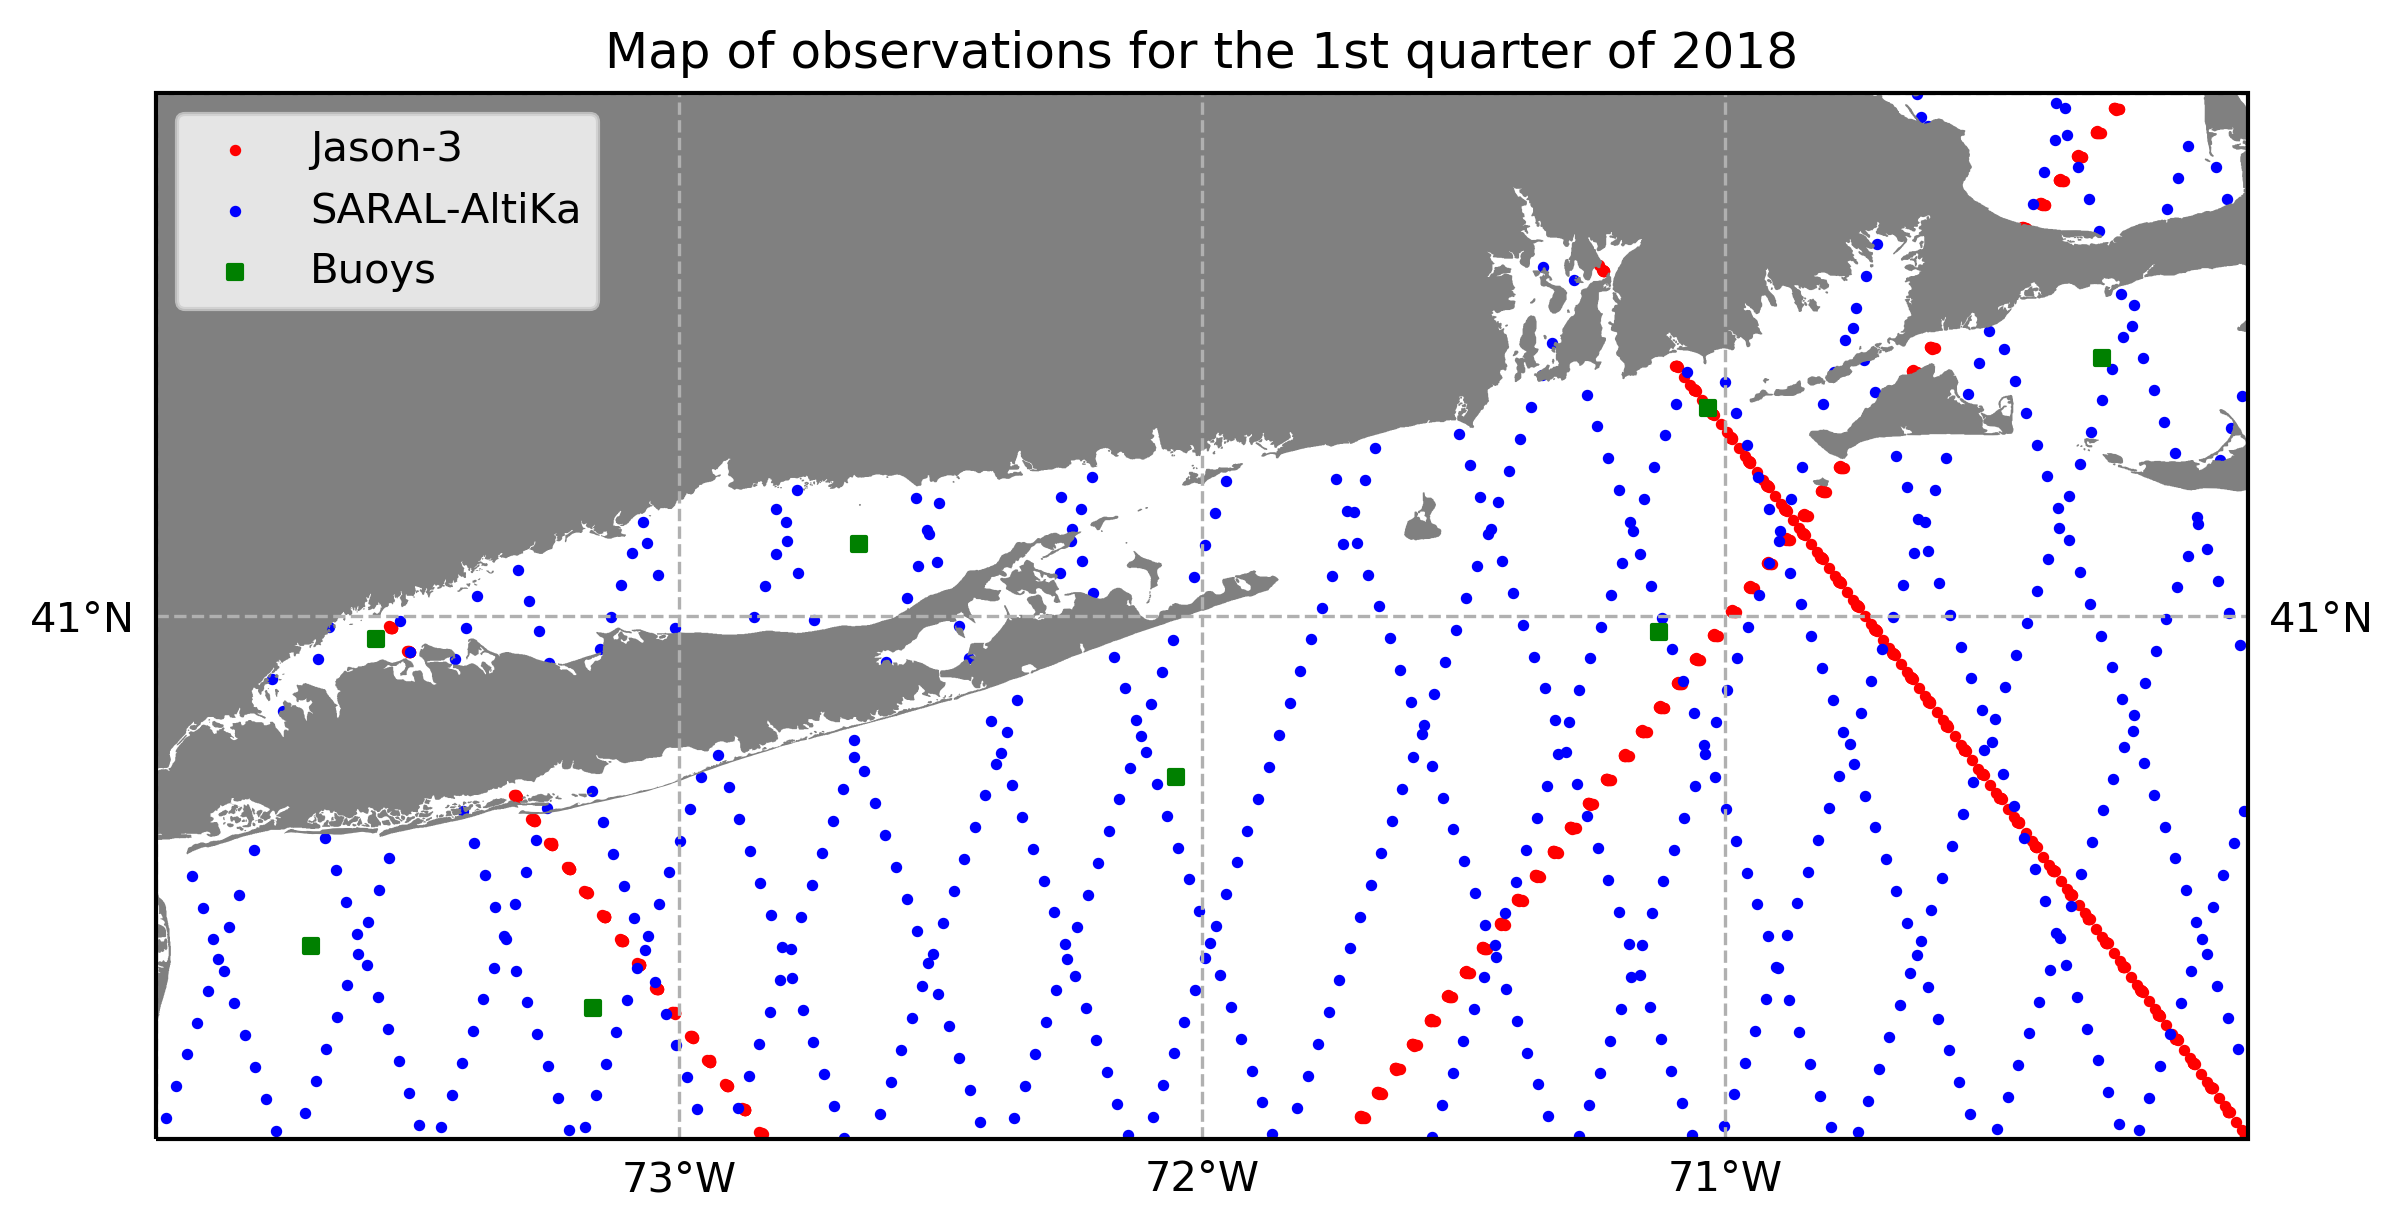
\includegraphics[width=\linewidth]{Figures/SNE_obs_q1_2018}
%\decoRule
\caption[Map of Observations for the 1st quarter of 2018]{An electron (artist's impression).}
\label{fig:SNE_obs_q1_2018}
\end{figure}

Sometimes figures don't always appear where you write them in the source. The placement depends on how much space there is on the page for the figure. Sometimes there is not enough room to fit a figure directly where it should go (in relation to the text) and so \LaTeX{} puts it at the top of the next page. Positioning figures is the job of \LaTeX{} and so you should only worry about making them look good!

Figures usually should have captions just in case you need to refer to them (such as in Figure~\ref{fig:SNE_obs_q1_2018}). The \verb|\caption| command contains two parts, the first part, inside the square brackets is the title that will appear in the \emph{List of Figures}, and so should be short. The second part in the curly brackets should contain the longer and more descriptive caption text.

The \verb|\decoRule| command is optional and simply puts an aesthetic horizontal line below the image. If you do this for one image, do it for all of them.

\LaTeX{} is capable of using images in pdf, jpg and png format.

\subsection{Typesetting mathematics}

If your thesis is going to contain heavy mathematical content, be sure that \LaTeX{} will make it look beautiful, even though it won't be able to solve the equations for you.

The \enquote{Not So Short Introduction to \LaTeX} (available on \href{http://www.ctan.org/tex-archive/info/lshort/english/lshort.pdf}{CTAN}) should tell you everything you need to know for most cases of typesetting mathematics. If you need more information, a much more thorough mathematical guide is available from the AMS called, \enquote{A Short Math Guide to \LaTeX} and can be downloaded from:
\url{ftp://ftp.ams.org/pub/tex/doc/amsmath/short-math-guide.pdf}

There are many different \LaTeX{} symbols to remember, luckily you can find the most common symbols in \href{http://ctan.org/pkg/comprehensive}{The Comprehensive \LaTeX~Symbol List}.

You can write an equation, which is automatically given an equation number by \LaTeX{} like this:
\begin{verbatim}
\begin{equation}
E = mc^{2}
\label{eqn:Einstein}
\end{equation}
\end{verbatim}

This will produce Einstein's famous energy-matter equivalence equation:
\begin{equation}
E = mc^{2}
\label{eqn:Einstein}
\end{equation}

All equations you write (which are not in the middle of paragraph text) are automatically given equation numbers by \LaTeX{}. If you don't want a particular equation numbered, use the unnumbered form:
\begin{verbatim}
\[ a^{2}=4 \]
\end{verbatim}

%----------------------------------------------------------------------------------------

\section{Sectioning and Subsectioning}

You should break your thesis up into nice, bite-sized sections and subsections. \LaTeX{} automatically builds a table of Contents by looking at all the \verb|\chapter{}|, \verb|\section{}|  and \verb|\subsection{}| commands you write in the source.

The Table of Contents should only list the sections to three (3) levels. A \verb|chapter{}| is level zero (0). A \verb|\section{}| is level one (1) and so a \verb|\subsection{}| is level two (2). In your thesis it is likely that you will even use a \verb|subsubsection{}|, which is level three (3). The depth to which the Table of Contents is formatted is set within \file{MastersDoctoralThesis.cls}. If you need this changed, you can do it in \file{main.tex}.

%----------------------------------------------------------------------------------------

\section{In Closing}

You have reached the end of this mini-guide. You can now rename or overwrite this pdf file and begin writing your own \file{Chapter1.tex} and the rest of your thesis. The easy work of setting up the structure and framework has been taken care of for you. It's now your job to fill it out!

Good luck and have lots of fun!

\begin{flushright}
Guide written by ---\\
Sunil Patel: \href{http://www.sunilpatel.co.uk}{www.sunilpatel.co.uk}\\
Vel: \href{http://www.LaTeXTemplates.com}{LaTeXTemplates.com}
\end{flushright}

% Chapter 2

\chapter{Theoretical Background} % Main chapter title

\label{Chapter2} % For referencing the chapter elsewhere, use \ref{Chapter2}

%----------------------------------------------------------------------------------------

\section{Significant Wave Height and Wave Spectra}\label{swh_spectra}

Historically, the study of wave growth and the interest in its prediction have their origins in the Second World War when it was critical for landing operations. Munk \cite{Munk2010} classified ocean waves according to their propagation period and documented the need for further comprehension of the wave spectrum. The band of the range of ocean waves that we are focusing on in this study is the ordinary gravity waves, as shown in Figure~\ref{fig:ocean_waves}. Wave characteristics that describe what we call sea state were first observed visually and empirically defined. Since then, a better understanding of the generation of waves and the need for reliable and continuous observations led to what we perceive as the SWH and wave spectrum nowadays.


\begin{figure}[H]
\centering
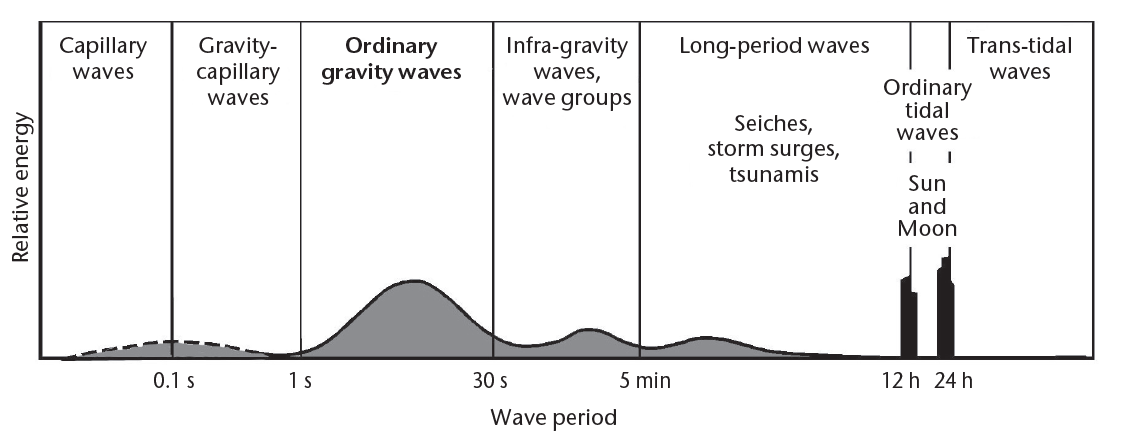
\includegraphics[width=0.95\linewidth]{Figures/Chapter2/ocean_waves.png}
%\decoRule
\caption{The classification of ocean waves depending on their period according to Munk \cite{Munk2010}. Reprinted from: \cite{Organization1998a}}
\label{fig:ocean_waves}
\end{figure}


First, we need to define the linear waves' fundamental parameters. The wavelength \emph{$\lambda$} is the horizontal distance between two consecutive crests of a wave in meters, and it is connected with the wavenumber \emph{k}, the number of crests per unit distance:


\begin{equation}
k = \frac{2\pi}{\lambda}
\label{eqn:wavenumber}
\end{equation}


Wave frequency \emph{f} is equal to the number of crests that pass from a point every second. Wave period \emph{T} is the time interval in seconds between the passage of successive crests from a fixed location. They are both related with the angular frequency \emph{$\omega$} in radians per second:


\begin{equation}
\omega = \frac{2\pi}{T} = 2\pi f
\label{eqn:angular_frequency}
\end{equation}

The wavenumber and wave frequency are connected with the dispersion relation, which characterizes wave propagation variation. The dispersion relation of ordinary gravity waves for specific depth \emph{h} is given by: 

\begin{equation}
\omega^{2} = gk\tanh{kh} 
\label{eqn:dispersion_relation}
\end{equation}

Other important parameters, especially for navigation and offshore installations, include the amplitude $\alpha$, which is the maximum displacement from the mean or zero sea level, and the wave height \emph{H}, which is the vertical distance of the successive troughs and crests, both measured in meters. Finally, we need to know the wave direction in degrees from which the waves propagate to characterize the sea state.

 
The definition of random ocean waves rests on the assumption that they are a superposition of an infinite number of components. Each wave component is characterized by a unique combination of frequency and propagation direction. The vertical displacement of waves in 2-dimensional space and time is given by the sum of the components' surface elevation \cite{Goda2010a}:
 
 \begin{equation}
\eta \left(x, y, t\right) = \sum_{n=1}^{\infty} \alpha_{n} \cos{\left(k_{n}x \cos{\theta_{n}} + k_{n}y \sin{\theta_{n}} - 2\pi f_{n}t + \epsilon_{n}  \right)}
\label{eqn:wave_elevation_3d}
\end{equation}
 
 Each wave component has a different phase angle \emph{$\epsilon_{n}$} between 0 and $2\pi$. The sum of the squared amplitudes of the wave components has a unique value:
 
\begin{equation}
\sum_{f}^{f+df} \sum_{\theta}^{\theta+d\theta} \frac{1}{2} \alpha^{2}_{n} = S\left(f,\theta\right)dfd\theta
\label{eqn:amplitude_spectrum}
\end{equation}
 
The function $S\left(f,\theta\right)$ is the directional wave spectrum, and it represents the wave energy distribution with respect to the different frequencies and directions of ocean waves because the squared amplitudes are also present at the wave energy equation:
 
\begin{equation}
E = \frac{\rho_{w}gH^{2}}{8} = \frac{\rho_{w}g\alpha^{2}}{2} 
\label{eqn:wave_energy}
\end{equation}

Where $p_{w}$ is the water density and \emph{g} is the gravitational acceleration constant. Therefore, a transformation of $S(f,\theta)$ to $p_{w}gS(f,\theta)$ is necessary first to be consistent with the energy spectrum term. The total wave energy is represented by $m_{0}$ which is the zeroth-moment of the spectrum \cite{Ardhuin2019a}, and it is calculated by the integral of the $S(f,\theta)$ function in all frequencies and directions:

\begin{equation}
m_{0} = \int_{0}^{\infty} \int_{0}^{2\pi} S(f,\theta) df d\theta
\label{eqn:total_wave_energy}
\end{equation}

This integral is by definition equal to the surface elevation variance $\overline{\eta^{2}}$. Thus, wave elevation variance is a more accurate term than wave energy. SWH is defined as four times the Root-Mean-Square (RMS) of the elevation variance, and it is denoted as \emph{$H_{s}$} or \emph{$H_{m0}$}.

\begin{equation}
H_{s} = 4\sqrt{m_{0}}
\label{eqn:swh_hs}
\end{equation}
 
 
 
When directional information is unavailable, we can obtain the wave spectrum as a function only of the frequencies. It becomes the frequency spectrum, an example of which is shown in Figure~\ref{fig:freq_spectrum} using buoy observations. The infinite number of wave frequencies are represented on the x-axis. In reality, sensors onboard buoys divide the whole spectrum into frequency bands with an \emph{f+df} size. NDBC uses frequency bands of 0.01 Hz size with a cut-in frequency of 0.03 Hz and a cut-off frequency of 0.4 Hz. On the other hand, CDIP uses narrower frequency bands of 0.005 Hz for a more extended spectrum with a cut-in frequency of 0.025 Hz and a cut-off frequency of 0.58 Hz. The elevation variances or the wave energies are plotted on the y-axis in $m^{2}s$ or $m^{2}/Hz$.


 
\begin{figure}[H]
\centering
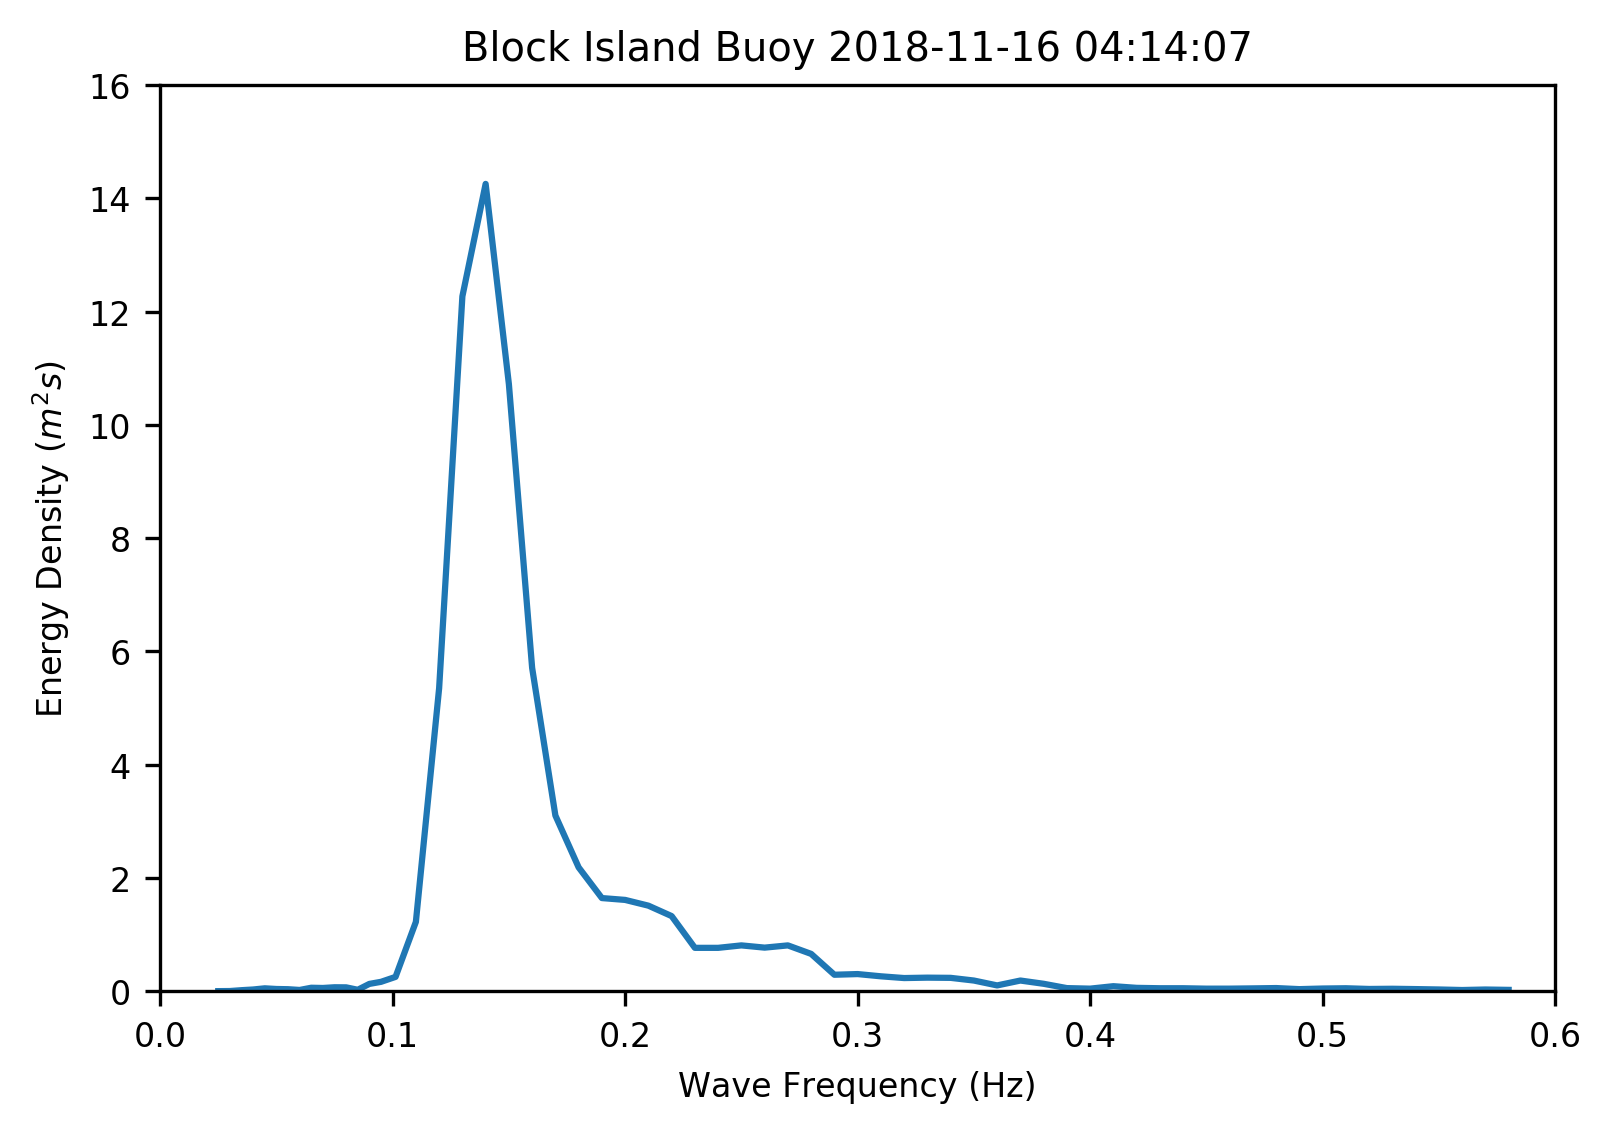
\includegraphics[width=0.85\linewidth]{Figures/Chapter2/freq_spectrum.png}
%\decoRule
\caption{An example of a wave frequency spectrum. Data presented were reported from Block Island buoy 44097 on October 27 2018.}
\label{fig:freq_spectrum}
\end{figure}


From the frequency spectrum, we can derive two primary parameters for our study, the SWH and the peak or dominant period $T_{p}$. The integral of the spectrum that represents the volume of the area under its continuous curve in Figure~\ref{fig:freq_spectrum} is equal to the zeroth-moment of the spectrum $m_{0}$, and it is the representative value of the total wave energy as defined in \ref{eqn:total_wave_energy}. Therefore, SWH is expressed as four times the square root of this integral. From the frequency spectrum, we can also derive the peak frequency $f_{p}$, which is the wave frequency of the spectrum's peak band. The wave dominant period $T_{p}$ corresponds to the peak frequency band.


To estimate SWH and $T_{p}$ from the wave spectrum accurately, observations are assumed to represent statistically stationary random processes. The aim is to prevent scattering of the observation values; hence, we need a relatively large wave measurement record \cite{Organization1998a}. To satisfy both conditions, NDBC and CDIP stations record raw 1 Hz observations for 20 minutes (see \ref{buoy_observations}).


The directional wave spectrum \emph{S(f,$\theta$)} is the distribution of the elevation variance or the wave energy both in the frequency domain and the wave components' direction. An example of the directional wave spectrum from buoy observations is shown in \ref{fig:dir_spectrum} and the wave energy density is reported in $m^{2}s/deg$ or $m^{2}s/rad$.


Except for the SWH and $T_{p}$, we also need information relative to the ocean waves' direction to obtain a complete picture of the sea state. Except for the surface elevation, buoys contain directional wave sensors measuring the slope vector, and they are included in their raw time series. These measuring systems are called heave pitch and roll, and the slope time series are measured in the east-west, and north-south direction using buoy azimuth \cite{Steele1998}. 
 
 
The directional wave spectrum is also expressed as:
 
 \begin{equation}
S(f,\theta) = S(f)D(f,\theta)
\label{eqn:amplitude_freqdir_spectrum2}
\end{equation}

where $D(f,\theta)$ is the directional spreading function:

\begin{equation}
\int_{-\pi}^{\pi} D(f,\theta)d\theta = 1
\label{eqn:directional_spreading}
\end{equation}

\emph{D(f,$\theta$)} describes how the wave energy density is spread in all directions. Longuet-Higgins \cite{longuet1963}, estimated the wave spectrum using the Fourier series methodology and proved that the first four coefficients are needed to describe the spectrum, including its directional parameters. The four Fourier coefficients are calculated by applying cross-spectral analysis to the wave elevation and the buoys' slope time series. This process is extensively described in \citep{Dean1991a, Earle1996, Earle1999, Kuik1988}.

\begin{figure}[H]
\centering
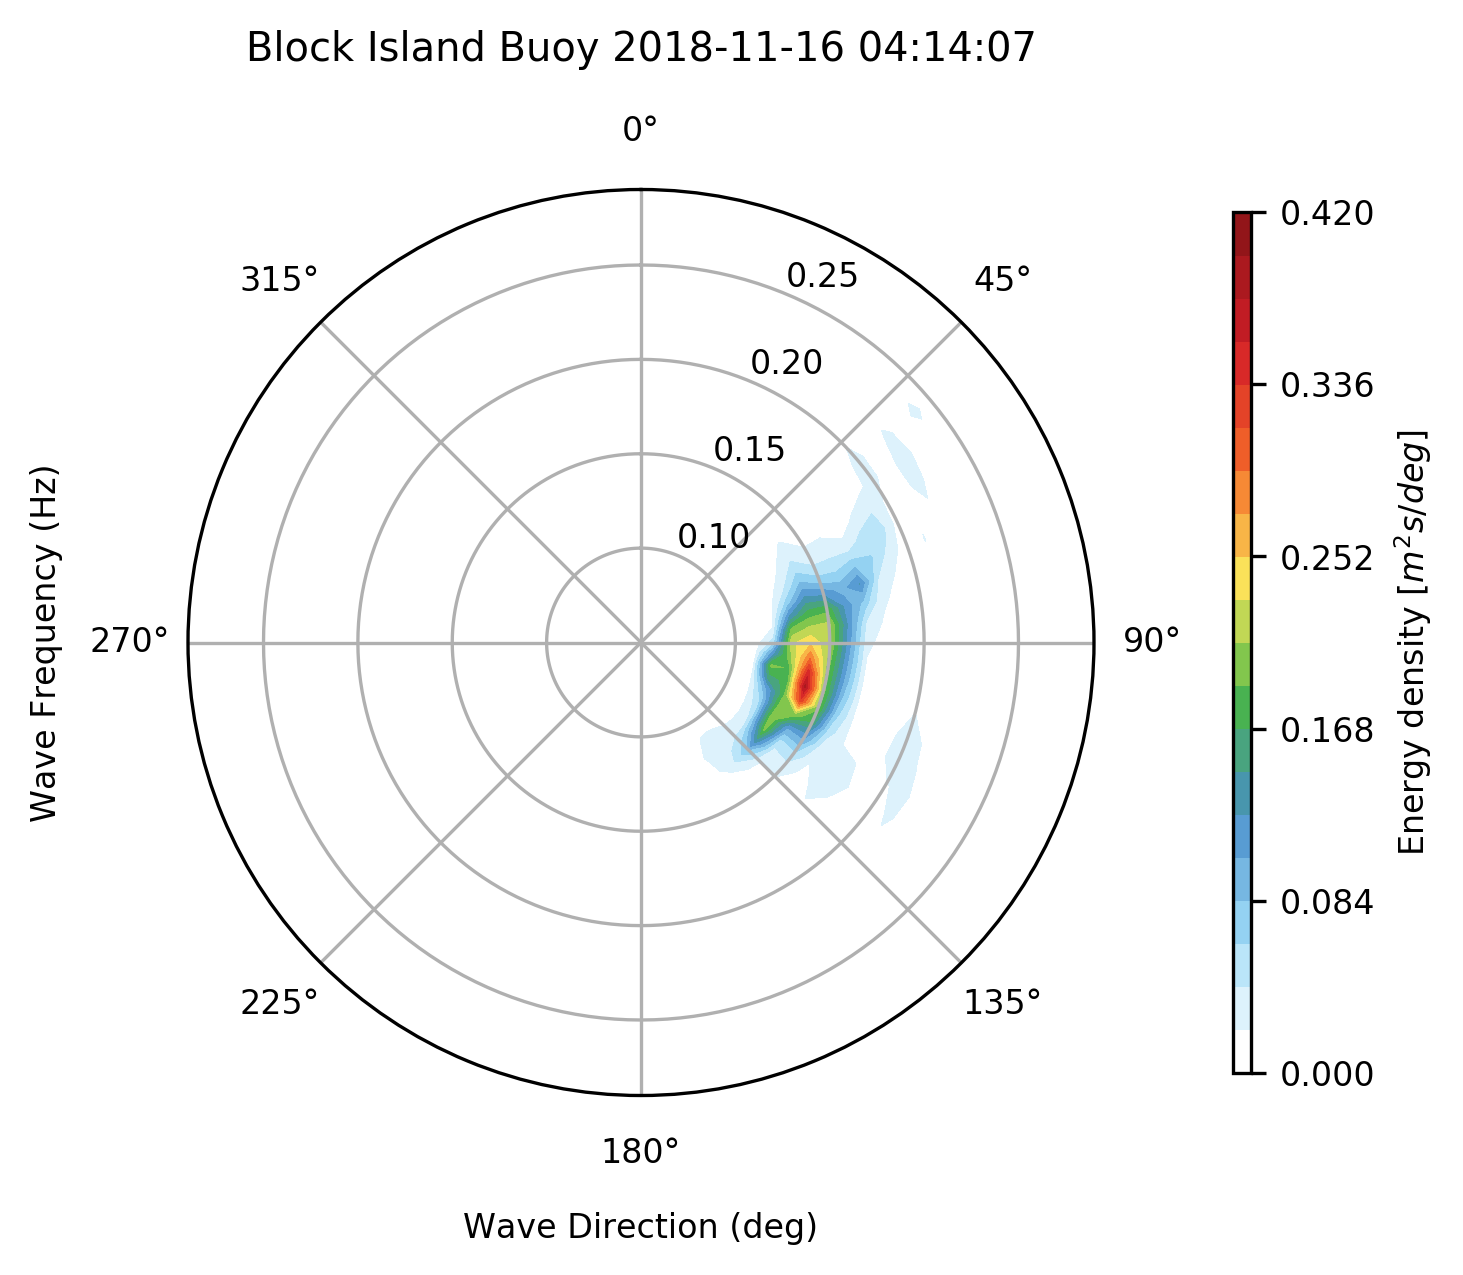
\includegraphics[width=0.85\linewidth]{Figures/Chapter2/dir_spectrum.png}
%\decoRule
\caption{An example of a wave directional spectrum. Data presented were reported from Block Island buoy 44097 for October 27 2018.}
\label{fig:dir_spectrum}
\end{figure}

The challenge is to reconstruct the directional spreading function from the estimated Fourier coefficients and create the directional spectra. It is worth mentioning that NDBC buoys, using the Datawell Hippy 40 sensor, measure and then disseminate the frequency spectrum and the four Fourier coefficient time series \cite{Steele1998}. Still, the final two-dimensional spectra are not provided. CDIP provides only recent directional spectra online. There are several methods to reconstruct the two-dimensional, directional spectra. The Maximum Entropy Method (MEM) \cite{Lygre1986}, is considered the most reliable \cite{Ardhuin2019a}. CDIP also uses this method to reconstruct the directional spectra. Its disadvantage is that often the spectrum's shape contains artificial double-peaks. An extended discussion of the various methods to reconstruct the directional spectrum is available in \cite{Earle1999, Goda2010c, Young1999a}.


%---------------------------------------------------------------------------


\section{Wave Age and Spectral Decomposition}\label{decomposition_waveage}


In the previous section, we discussed the importance of the directional wave spectra to describe the ocean wave conditions. We also emphasized that the waves contributing to the wave spectrum have various frequencies, directions, heights, and periods. This leads us to study waves according to their unique characteristics and influence on the wave climate. 

Waves can be classified according to their growth status. Local waves that owe their development to the increasing momentum input from the wind are called wind waves or wind sea. When the wind speed is reduced, and the wind's relative direction with the waves is increased over 30 degrees, or when remotely-generated waves due to a distant storm arrive, they are called swell \cite{Organization1998a}. Wind waves  are strongly correlated with the wind, and they have a notable presence during extreme events, in enclosed basins, and coastal regions. An empirical method often used is to classify waves as wind sea when their dominant period has a duration of fewer than 10 seconds. In contrast, swells are not coupled with the wind, and they do not owe their development to a local wind momentum input. Besides, swell waves are different visually, as they appear as more organized groups of waves with smoother crests. In this study, we will focus on two methods of ocean wave classification.

The first method is based on ocean waves' growth using the inverse wave age criterion \cite{Hanley2010}. Wave age $c_{p}/U_{10}\cos{\theta_{d}}$ represents the wind's potential to transfer energy to the waves \cite{Zhao2019}. $c_{p}$ is the wave phase speed at the peak of their spectrum and it is equal to $\lambda_{p}/T_{p}$ or $\omega_{p}/k_{p}$. Once wind-waves are generated, the wind is faster than the waves. As the energy is provided to the wind waves, their celerity increases until they reach the wind-wave equilibrium, at which the sea is considered mature or fully developed:


\begin{equation}
\frac{c_{p}}{U_{10}\cos{\theta_{d}}} = 1.2
\label{eqn:wave_age}
\end{equation}

$u_{10}$ is the wind speed at 10 meters height, which is discussed in the next Section~\ref{WindProfile} and $\theta_{d}$ is the relative angle between the wind direction and the mean wave direction. 
If we combine $c_{p}$ with the dispersion relation for deep water waves $\omega^{2} = gk$ and \ref{eqn:angular_frequency}, the result is a relationship which connects the peak propagation speed with the dominant period \cite{Hanley2010}:

\begin{equation}
c_{p} = \frac{gT_{p}}{2\pi}
\label{eqn:peak_wave_speed}
\end{equation}


The inverse wave criterion is used to classify waves from buoy time series as in similar studies \cite{DeFarias2012a, Hanley2010}. We classify wind waves according to the following condition:

\begin{equation}
\frac{U_{10}\cos{\theta_{d}}}{c_{p}} > 0.83
\label{eqn:inv_wave_age}
\end{equation}

The remaining waves are considered swell or mixed seas. An advantage of current sensors onboard boys is that both wind and mean wave direction are measured. Therefore, we can add an intermediate range for mixed sea states 0.15 < $U_{10}cos{\theta_{d}}/c_{p}$ < 0.83 \cite{Hanley2010}. It is worth mentioning that these are not hard limits, though. 

\vspace{4mm} 

The second way to classify ocean waves is more advanced and relies on the wave directional spectra. This method is called spectral partitioning, and it is implemented for the spectral decomposition of waves to wind sea and swell partitions. An example of a directional spectrum is shown in \ref{fig:dir_spectrum}. This figure shows a single system describing the sea state. A common condition, especially in the open ocean, is to have multiple systems with unique frequencies coming from diverse directions. One of the main benefits of spectral partitioning is to decompose the different systems into wind waves and swells operationally in numerical models \cite{Organization1998a}. NDBC does not disseminate historical partitioned data for wind waves and swells. It recommends empirical methods \cite{Gilhousen2001} that rely on the determination of the separation frequency $f_{s}$, which separates the different wave systems.

For this study, we use a Matlab algorithm \cite{Douglas2019} to partition wind wave and swell systems during extreme events (see \ref{results}). This algorithm is mainly based on the \emph{watershed} methodology described in \cite{Hanson2001a}. With this method, the different watershed regions are identified from the input directional spectrum matrix, and then they are assigned a number that differentiates each system from the other. A similar algorithm is used operationally for the spectral partitioning in the \emph{Wavewatch III} (WW3) model \cite{WW2019a}. There are also other spectral partitioning methods. Wang and Hwang \cite{Wang2001} use a spectral steepness method which utilizes the peak frequency to calculate the separation frequency without taking into account the wave direction. Portilla et al. \cite{Portilla2009} propose a different methodology also based on the watershed algorithm.



%----------------------------------------------------------------------------------------

\section{Sea surface roughness and the wind speed profile over the ocean}\label{WindProfile}


To quantify the interaction between the atmosphere and the ocean, we need to measure the exchange of momentum at the sea surface. This exchange's direct measurement is not an easy task, though; therefore, oceanographers and meteorologists estimate it through bulk formulas. Precisely, the flux of momentum is quantified by the wind stress on the ocean surface:

\begin{equation}
\tau = \rho_{a} u_{*}^{2}  = \rho_{a}  C_{D} U_{r}^{2}
\label{eqn:wind_stress}
\end{equation}

where $\rho_{a}$ is the density of air, $U_{r}$ is the wind speed relative to the speed of the water and $C_{D}$ is the drag coefficient \cite{Edson2013}. $u_{*}$ is the friction velocity. While $\rho$ and $U_{r}$ can be directly measured, $C_{D}$ is a subject of many theoretical and experimental  parameterizations. The theoretical parameterization of the drag coefficient is derived from the Monin-Obukhov similarity theory:

\begin{equation}
C_{D} = \left( \frac{k}{\ln{z/z_{0}} - \psi_{m}(z/L)} \right)^2
\label{eqn:cd_non_neutral}
\end{equation}

where $k=0.4$ is the Von Karman constant, $z_{0}$ is the roughness length, $\psi_{m}$ is a dimensionless function that controls the stability of the atmosphere. Besides, \emph{z} is the reference height where we want to estimate the drag coefficient, and \emph{L} is the Monin-Obukhov length. A thorough description of the drag coefficient's dependency on atmospheric stability is available in \cite{Smith1988}, including examples for different conditions. 


For an accurate estimation of $C_{D}$, it is necessary to obtain observations of WS, air and water temperature, and humidity, among other parameters. In practice, as is the case for NDBC buoy observations, all these parameters are not always available because they are measured from different sensors. Hence, only dedicated experiments on air-sea interaction provide all the necessary information to assess the air-sea coupling. For this reason, the stability function is often eliminated, and we assume neutral stability of the atmospheric boundary layer over the ocean. A quantification of the errors that this assumption creates is presented in \ref{fig:stability}. Under neutral boundary layer conditions, the wind speed logarithmic profile over the ocean is described by:

\begin{equation}
u_{z} = \frac{u_{*}}{k} \ln\left({\frac{z}{z_{0}}}\right)
\label{eqn:log_profile}
\end{equation}

Combining the latter equation and \ref{eqn:wind_stress}, we can estimate the wind speed at the reference height of 10 meters ($u_{10}$) given the wind speed at a different height, the drag coefficient and the roughness length \cite{Young1999b}. 


\begin{equation}
u_{10} = u_{z} \frac{k}{\sqrt{C_{DN}}} \ln^{-1}\left({\frac{z}{z_{0}}}\right)
\label{eqn:u10}
\end{equation}

NDBC does not report the wind speed at 10 meters, though. It suggests two different ways of adjusting the WS at a reference height \cite{Hsu1994a, Liu1979}. The latter method is based on the power-law wind profile mainly used for the WS adjustment over land, and offshore wind design \cite{Commision2019}. A comparison of the logarithmic and the power-law \cite{Emeis2013} has shown that for values of the wind shear coefficient that approach the ocean surface conditions, the difference between them is minimal and gets even smaller as we go higher in the atmosphere and inside the surface layer (80-100 meters). 
 
\begin{figure}[H]
\centering
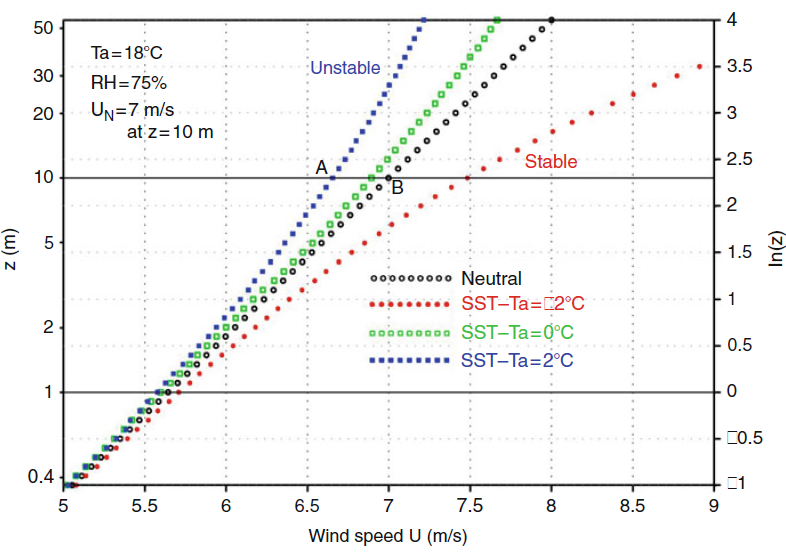
\includegraphics[width=0.75\linewidth]{Figures/Chapter2/stability.png}
%\decoRule
\caption{The influence of the neutral stability assumption in various conditions and heights near the sea surface. Point B represents the wind speed at 10 meters under neutrally stable conditions and A the measured value. Derived from: \cite{Liu2014}}
\label{fig:stability}
\end{figure}

We also define the drag coefficient at 10 meters height for a neutrally stable atmospheric boundary layer using \ref{eqn:cd_non_neutral}:


\begin{equation}
C_{DN10} = \left( \frac{k}{\ln{\left( 10/z_{0} \right)}} \right)^2
\label{eqn:cd_neutral}
\end{equation}

In this case, it is evident that estimating $C_{D}$ means that we can estimate the $z_{0}$. The roughness length over the ocean is not constant and dependent on the sea state. There are proposed methodologies to predict the roughness length from the wave age and SWH \cite{Taylor2001}. An extensive literature review of the most popular drag coefficient and roughness length parameterizations is available in the literature \cite{Bryant2016, Zhao2019}. The latter also explores the parameterization of $C_{D}$ and $z_{0}$ using the wave age and the wave steepness ($H/\lambda$). As the surface wind increases until the ocean surface gets fully rough, the wind stress strengthens its impact, and $C_{D}$ has higher values. Although it is true for moderate to high winds, it has been proven that the linear increase of the drag coefficient with increased wind speed does not apply for low wind speeds.  During conditions of very low winds ($u_{10} < 4 m/s$)  and the presence of aligned with the wind direction swells, the momentum flux reserves its sign from positive to negative, and the assumption of a neutrally stable, logarithmic profile over the sea surface is no longer valid \cite{Edson2013, Grachev2001, Hanley2008}.

From the number of available parameterizations, it is evident that the task to describe the air-sea interactions sufficiently is multi-faceted. This study uses a specific parameterization while considering the errors therein and the possible deviations from the truth. Specifically, we use equation \ref{eqn:u10} to adjust the reported wind speed observations from the buoys to the reference height of 10 meters. Representative values of $C_{D} = 1.2 \times 10^{-3}$ and the corresponding $z_{0} = 9.7 \times 10^{-5} m$ derived from \ref{eqn:cd_neutral} are also used in similar studies \cite{Ribal2019, Young2017}. Anemometers onboard buoys are placed on various heights (3.5 to 4.5 meters) depending on the buoy type. Hence, adjusting to a reference height is also beneficial for consistent comparisons.



%----------------------------------------------------------------------------------------


\section{Literature  review  of  bulk  formulae  for  wind-wave  relationships}\label{wind_wave_relationships}


In the first section of this Chapter \ref{swh_spectra}, we showed that SWH is estimated from the frequency spectrum and it is equal to four times the integral of the area under the continuous line of the spectrum, or the RMS elevation.

Historically, WS and SWH relationships are synonymous to the wave spectrum. Pierson's spectrum approach to ocean waves \cite{Pierson1955} was transcedental as he developed the theoretical background and the statistics of ocean wave spectra. Neumann implemented Pierson's theory and created the first wave spectrum using visual wave observations from ships. The Neumann spectrum was the first to connect the WS at the height of the anemometer as a driving force for the waves with the frequency spectrum. The fully developed or fully aroused sea was then defined as the sea state with a spectrum of all frequency components with the maximum energy under a specific value of WS forcing. This led to the SWH definition and the first relationships of SWH and WS based on the wave spectrum of a fully developed sea. The first three relationships came from the Pierson-Neumann system of equations \ref{eqn:pierson_neumann}, the  Sverdrup-Munk-Bretschneider wave forecasting method \ref{eqn:sverdrup_munk} and the Darbyshire spectrum \ref{eqn:darbyshire}. 

\begin{equation}
H_{s} = 7.065 \times 10^{-6} u^{2.5}
\label{eqn:pierson_neumann}
\end{equation}

\begin{equation}
H_{s} = 2.667 \times 10^{-4} u^{2}
\label{eqn:sverdrup_munk}
\end{equation}

\begin{equation}
H_{s} = 1.39 \times 10^{-4} u^{2}
\label{eqn:darbyshire}
\end{equation}

A comparison of theoretical spectra and their corresponding wind-wave relationships is available in \cite{Neumann1957}.

Kitagorodskii based on the Pierson-Moskowitz spectrum \cite{Pierson1964}, proposed similar empirical laws for the fully-developed sea. One of Kitagorodskii's empirical formulas is also the wave age wind-wave equilibrium equation \ref{eqn:wave_age}. For the fully-developed sea, he connected $u_{10}$ with $H_{s}$ \cite{CsanadyASI2001}:

\begin{equation}
H_{s} = \frac{0.2}{g} u_{10}^{2}
\label{eqn:kitagorodskii}
\end{equation}

A few years later, Carter \cite{Carter1982} reviewed the JONSWAP spectrum \cite{Hasselmann1973} and proposed the following relationship:

\begin{equation}
H_{s} = 0.02466 u_{10}^{2}
\label{eqn:jonswap}
\end{equation}

This relationship is also used as a reference in similar and contemporary studies \cite{Andreas2007}. Carter also proposed equations for the duration and fetch-limited seas:

\begin{equation}
H_{s} = 0.0163 X^{0.5} u_{10}
\label{eqn:fetch_limited}
\end{equation}

\begin{equation}
H_{s} = 0.0146 D^{5/7} u_{10}^{9/7}
\label{eqn:duration_limited}
\end{equation}

The sea is considered duration-limited when:

\begin{equation}
D > 1.167 X^{0.7} u_{10}^{-0.4}
\label{eqn:duration_limited_condition}
\end{equation}

\emph{X} is the fetch, the perpendicular distance to the upwind coast in kilometers and \emph{D} is the duration in hours. In this study, fetch is not included directly in the estimations. However, we examine the relationships for each of the main wind directions to indirectly connect them with the variation of the fetch in coastal regions.

WMO \cite{Organization1998a} suggests a similar empirical relationship for the estimation of SWH when $u_{10}$ is given.

\begin{equation}
H_{s} = \left(\frac{u_{10}}{12.5}\right)^{2}
\label{eqn:wmo_relationship}
\end{equation}

Finally, other studies incorporate wind-wave relationships from wave models for classification of the sea state into wind-waves and swells using altimeter data \cite{Chen2002}.

All the relationships mentioned above are valid under the assumptions of deep water waves and fully developed seas. Consequently, SWH cannot be accurately estimated from $u_{10}$ in all other growth stages or with presence of swells. 



%----------------------------------------------------------------------------------------


\section{Wind Speed Probability Density Functions}\label{wind_wave_pdfs}


This section is about the statistical interpretation of the long-term time series from the buoys. Specifically, the ultimate goal is to indicate the Probability Density Functions (PDF) that describe the $u_{10}$ distribution as it is estimated from the buoy records for each location.

Wind PDFs are required for design assessment at the offshore wind farm site before its installation \cite{Commision2019}. They are an integral part of the wind data analysis, and they are usually combined with the wind roses that provide the directional distribution of the wind speed \cite{DNVGL2018}. The average wind turbine
power is also associated with the PDF estimation \cite{Morgan2011}. For the wind PDF estimation, the suggested buoy dataset is the 10-minute average $U_{10}$. Although the modern wind turbine hub heights are greater than or equal to 100 meters, an extrapolation of the surface WS to such height would result in high uncertainty \cite{Ng2016}. Therefore, a reference height of 10 meters is selected for this study. The results would also prove useful as a reference to a similar estimation of the PDFs from wind lidar buoy and offshore wind tower observations in a later stage.

The standard and most widely-accepted wind speed distribution is the Weibull:


\begin{equation}
f(x) = \alpha x^{\alpha-1} exp\left( - x^\alpha \right)
\label{eqn:weibull_2p}
\end{equation}

Where $\alpha>0$ is the shape parameter. The best fit to our data is the 3-parameter Weibull though, for $y = (x-\gamma)/\eta$, where $\eta$ is the scale and $\gamma$ is the location parameter. Special cases of the Weibull are the Exponential ($\beta = 1$) and the Rayleigh ($\alpha = 2$) distributions.

There also regional characteristics of the wind speed distribution. Previous studies using buoy data have proved that the Weibull distribution is adequate for estimating the surface wind PDFs only for specific regions \citep{Morgan2011}. They propose that universal models should be a mixture of multiple distributions with different assigned weights for each distribution, depending on the domain. There are also studies suggesting that the Johnson $S_{B}$ \cite{Soukissian2013, Soukissian2014} distribution can be accepted as an alternative PDF and the best fit for certain regions. As described in the results, we identify and evaluate four distribution with the best fit for the WS data in SNE. Two of them, Weibull and Rayleigh are already referenced above. Besides, the Beta and Johnson $S_{B}$ distributions are also suggested to describe the long-term WS distribution at SNE:


\begin{equation}
f(x) = \frac{\Gamma\left(\alpha+\beta\right)}{\Gamma(\alpha)\Gamma(\beta)} x^{\alpha-1}(1-x)^{\beta-1}
\label{eqn:beta}
\end{equation}

This is the Beta 2P distribution where $\Gamma$ is the Gamma function and $\alpha > 0$, $\beta > 0$ are the shape parameters. We evaluate the 4P Beta PDF by adding scale and location parameters for $y = (x-\gamma)/\eta$, where $\eta$ is the scale and $\gamma$ is the location parameter respectively.


\begin{equation}
f(x) = \frac{b}{x(1-x)} \phi\left(\alpha+\beta\log{\frac{x}{1-x}}\right)
\label{eqn:johnsonsb}
\end{equation}


This is the Johnson $S_{B}$ 2P distribution where $\alpha > 0$, $\beta > 0$ are the shape parameters and $\phi$ is the normal distribution PDF. We evaluate the 4P Johnson $S_{B}$ PDF by adding a scale and location parameters for $y = (x-\gamma)/\eta$, where $\eta$ is the scale and $\gamma$ is the location parameter respectively.


We identify the single, univariate distributions of best fit to the long-term $u_{10}$ time series using the extended \emph{SciPy} library of PDFs for each buoy location. This library utilizes the Maximum Likelihood Estimation (MLE) methodology for fitting to the theoretical distributions and the estimation of the distribution parameters.


%----------------------------------------------------------------------------------------



\section{Principles of Satellite Altimetry}\label{AltimetryPrinciples}

The Radar altimeter is an active, nadir looking microwave instrument that emits its impulses to the earth's surface. Once it receives them back, it measures the travel time, the magnitude, and the shape of each return signal.

The average of hundreds of pulses shape the mean returned signal. Specifically, the signals tracked originally by the altimeter are convolved to a single waveform after being fitted to a mathematical model. These function fitting methods are evolving through the years and are described in \cite{Gommenginger2011}. The process is fundamental for satellite altimetry and constitutes the retracking model. The mathematical model used for the fitting of the retracking algorithm is the Brown-Hayne model \cite{Brown1977TheApplications, Hayne1980RadarScattering} for the Low-Resolution Mode (LRM) and the SAMOSA model for the Synthetic Aperture Radar (SAR) altimetry \citep{Ray2015SARModel}. As a result, a typical waveform in the open ocean has three distinct areas, as presented in Figure~\ref{fig:altimeter_waveform}. The first one is the area of low, close to zero power. The second is the leading edge, which contains the area from the time that the waveform's power begins to increase until its peak. The third is the trailing edge, which is the area of decaying power of the waveform.

Except for the impulses' signal, an accurate determination of the earth's orbit is critical, especially the radial component. In addition, the target accuracy of the distance between the satellite and the sea level is on the order of 1 centimeter. Therefore, corrections due to the errors caused by the signal's delay as it travels through the ionosphere and the atmosphere have to be applied. The ionospheric corrections are essential to measuring the delay of the altimeter signal's travel time caused by the ionosphere's free electrons. It is also one reasons why a dual-frequency (Ku or Ka and C band) altimeter instrument is needed onboard the satellite. Besides, there are two kinds of atmospheric corrections: the dry tropospheric and the wet tropospheric correction. For the latter, the microwave radiometer instrument is used to measure the water vapor in the atmosphere. A significant challenge for coastal altimetry is that the microwave radiometer footprint radius is close to 50 kilometers. Therefore, the brightness temperature of the land contaminates the measurement in coastal areas. The wet troposphere correction is also very challenging due to the spatiotemporal variability of water vapor in the atmosphere. For these reasons, the uncontaminated signal in the open ocean is used in conjunction with in situ observations, when and where available, to correct the wet troposphere delay. Furthermore, there is uncertainty also at the surface of the ocean. Specifically, geophysical adjustments have to be applied to estimate parameters such as the earth and ocean tides, the sea state bias, and a dynamic atmosphere correction.

In coastal altimetry, the retracking model's fitting to get the final waveform has additional challenges as we get closer to the coast. Due to the extended radius of the altimeter footprint, land intrudes in the received signal, and there is land contamination of the waveform \citep{Halimi2013}. Hence, the final waveform can be corrupted, especially in high sea state conditions. Secondly, as we get closer to the coast, the footprint's backscatter is different from the one in the open ocean. Indeed, in coastal areas, the altimeter footprint may cover both a windy area with considerable sea surface roughness and an area of calm sea state with an almost flat surface “shaded” by the wind. As a result of the limitations mentioned above, the final waveform shows unusually higher power peaks in the trailing edge, a part of the waveform that we should otherwise not consider when fitting to the model to estimate the geophysical parameters.


\begin{figure}[H]
\centering
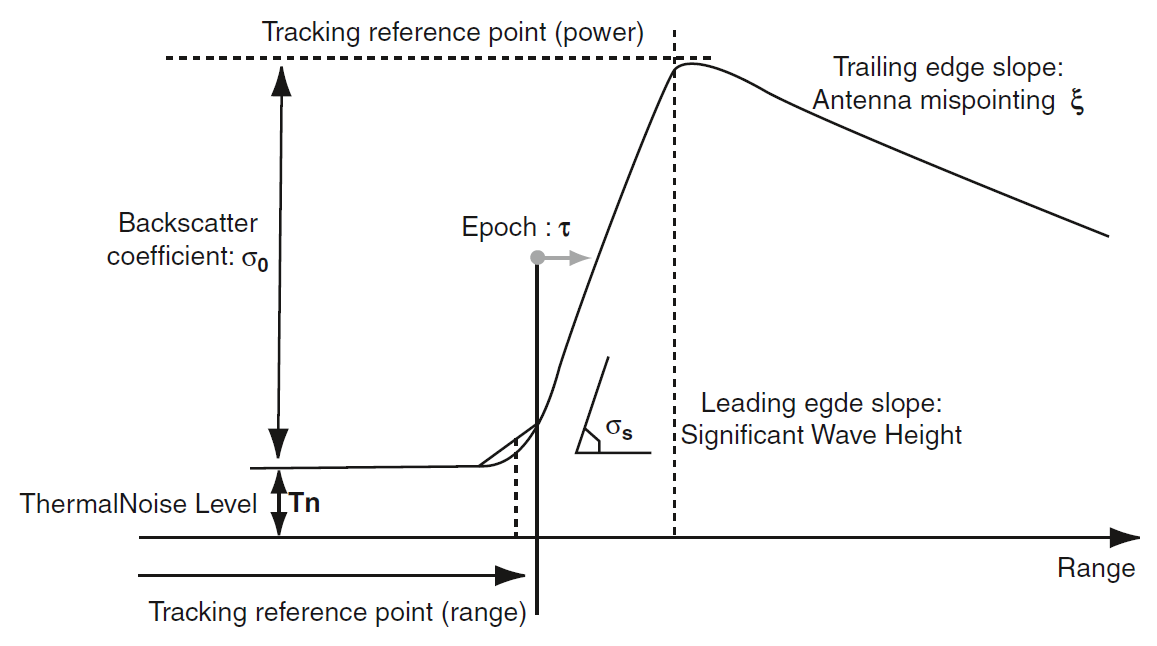
\includegraphics[width=0.85\linewidth]{Figures/Chapter2/altimeter_waveform.png}
%\decoRule
\caption{The Brown theoretical retracking model for LRM altimetry and the derived parameters. Derived from: \cite{Gommenginger2011}.}
\label{fig:altimeter_waveform}
\end{figure}



These limitations are evident when we consider the pulse-limited signal of the LRM altimeters. The effective footprint of the LRM altimeter is given by:

\begin{equation}
f = \frac{\pi R_{0} (c\tau + 2 H_{s})}{1 + R_{0}/R_{E}}
\label{eqn:effective_footprint}
\end{equation}

Where \emph{c} is the speed of light, \emph{$\tau$} is the pulse length, $H_{s}$ the SWH, $R_{0}$ the altitude of the satellite and $R_{E}$ the Earth's radius.

When the sea is calm, the altimeter's footprint is approximately a 2-kilometer radius in both directions, the along-track and the across-track. In contrast, during a storm or high sea state, the effective footprint can extend to over 7 kilometers. The principles of pulse-limited altimetry are extensively described in \cite{Chelton2001}. SAR or delay-Doppler altimetry using the Ray et al. \cite{Ray2015SARModel} model, revolutionized how the signal's power is used. On the one hand, it considers both the leading and the trailing edge of the retracked waveform instead of the smaller area of the leading edge considered for the LRM. The finer resolution on the along-track and the waveform's reduced noise are the main aspects of the evolution of SAR altimetry \cite{KeithRaney1998}. Its Pulse-Doppler-limited footprint's resolution can be constrained to approximately 300 meters only on the along-track. On the across-track, though, the resolution remains similar to the pulse-limited LRM. The effective footprint of SAR looks like slices of the LRM circular footprint as in Figure~\ref{fig:SAR_LRM}. The SAR altimetry pioneer is Cryosat 2 satellite, as it is equipped with the SIRAL instrument that operates in both modes (see \ref{altimeter_data}). Raynal et al. \cite{Raynal2018} demonstrates the increased accuracy of the SAR's higher spatial resolution over different areas worldwide. The European Space Agency (ESA) Sentinel 3 twin satellites, A and B, are the first missions that use the SAR altimetry mode exclusively. Currently, the remaining altimeters in orbit are operating in LRM mode. On the other hand, SARAL-AltiKa is the only LRM altimeter that emits its impulses in higher frequency using the Ka-band, which increases the accuracy of the measured parameters and reduces the noise of the final waveform.


 
\begin{figure}[H]
\centering
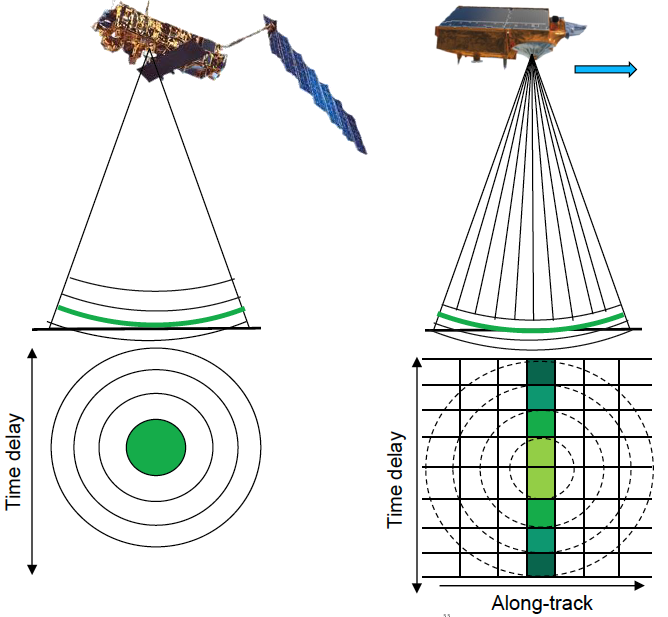
\includegraphics[width=0.8\linewidth]{Figures/Chapter2/sar_vs_lrm.png}
%\decoRule
\caption{A representation of the LRM and SAR altimeter footprint.}
\label{fig:SAR_LRM}
\end{figure}


We can determine at least three essential parameters from the retracked waveform \ref{fig:altimeter_waveform}. The first one is the epoch. We can then estimate the range from the epoch, which is the signal's travel time, until it reaches back the satellite and is connected with the Sea Surface Height (SSH). The second important parameter of the waveform is the slope of the leading edge (or width or rising time of the leading edge), which is connected to the estimation of the SWH. The third essential parameter is the backscatter coefficient derived by the received signal's power and is associated with the surface WS. For this study, the focus is on two of the three aforementioned geophysical parameters and their corresponding estimates, namely the SWH and the WS.

As previously discussed, the estimation of the SWH is connected with the slope of the leading edge. Specifically, the slope is a function of the root mean square error of the SWH. A steep leading edge represents a small value of the SWH. In contrast, for higher values of SWH, for example, during a storm, the return signal starts to rise earlier until it reaches its peak power, and also, the shape of the echo is different \cite{Ardhuin2019}. The difference between the two resulting waveforms, one during a calm sea and one for a rougher sea surface, is shown in Figure~\ref{fig:swh_altimeter}(b). It is evident that SWH from altimeters is derived with an entirely different measurement method with respect to buoys described in Chapter~\ref{swh_spectra}.


The radar altimeter also measures the backscatter signal's strength. This value is inversely proportional to the sea surface Mean Square Slope (MSS) \cite{Cox1954} which is related to the sea surface roughness induced by the wind. Therefore, the estimated WS increases as the surface MSS gets higher and the backscatter becomes smaller. The main source of errors in the altimeter estimation of the WS is the empirical nature of the corresponding algorithms that do not consider the impact of the sea state growth, primarily due to swells \cite{Abdalla2007, Glazman1990}. The retracking of hundreds of noisy signals and the need for reliable atmospheric corrections, notably close to the coast, makes the task even more challenging.



\begin{figure}[H]
\centering
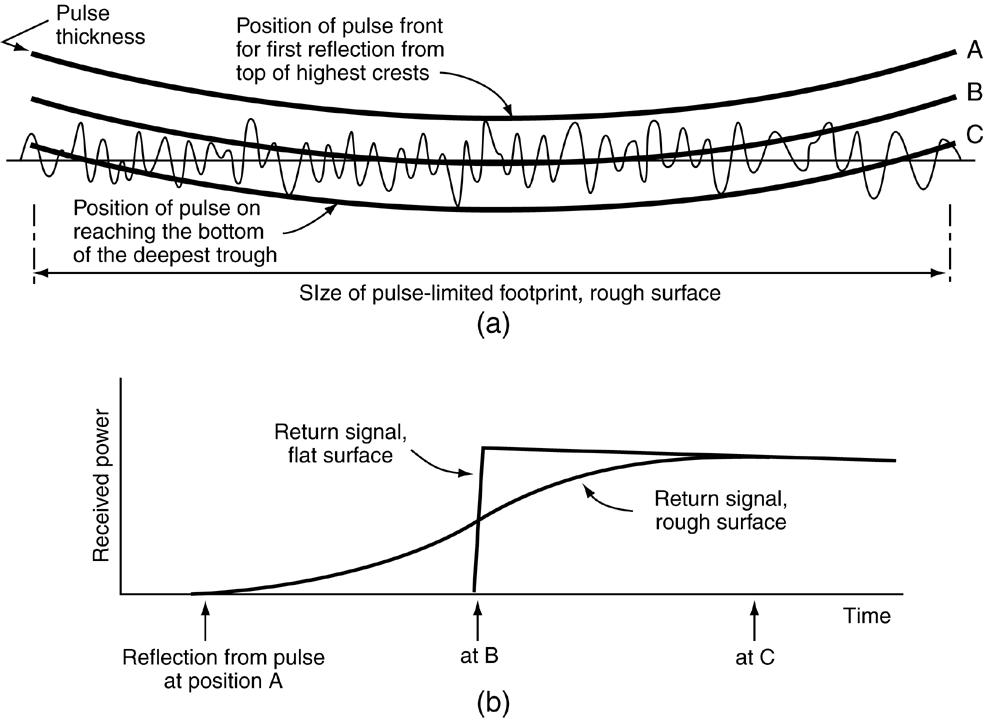
\includegraphics[width=0.8\linewidth]{Figures/Chapter2/swh_altimeter.png}
%\decoRule
\caption{(a) Illuminated surface geometry. (b) The resulting shape of the reflected pulse. Derived from: \citep{Robinson2010}}
\label{fig:swh_altimeter}
\end{figure}






%----------------------------------------------------------------------------------------



 
%% Chapter 4

\chapter{Methodology} % Main chapter title

\label{Chapter4} % For referencing the chapter elsewhere, use \ref{Chapter4}

%----------------------------------------------------------------------------------------

\section{Data preprocessing}

This study is based on the interpretation of wind and wave conditions using in situ and remote sensing observations from buoys and altimeters. There are fundamental differences in how in situ platforms measure and report the geophysical parameters compared to observations from satellite altimeters. On the one hand, buoys' measurements are considered the "ground truth", owing to their ability to provide a reliable, long-term, and continuous time-series record of temporally processed oceanographic and meteorological parameters from the raw data for a specific location. On the other hand, altimeters provide instantaneous measurements representing their sea surface footprint with a low temporal resolution. A description of satellite coastal altimetry challenges is available in \ref{AltimetryPrinciples}. 

This chapter aims to provide an outline of the collection and preprocess of the different data types. This step is essential because both datasets contain inherent and unique sources of error \cite{Glazman1990, Monaldo1988, Zieger2009}, and they need to be quality controlled before the analysis. The next step is to accurately describe the methodology that was implemented to achieve our final results. 


%-------------------------------------------------------------------------------------------


\subsection{Buoy Data Collection and Organization}\label{buoy_observations}

The importance of an extended and well-preserved network of buoys in the United States of America is well documented in \cite{Castellini2011}. This study utilizes all the wind and wave geophysical parameters reported by multiple stations of the NDBC and CDIP. CDIP is operated by the Ocean Engineering Research Group (OERG), part of the Integrative Oceanography Division (IOD) at Scripps Institution of Oceanography (SIO), and it is responsible for the operation and maintenance of buoys 44097 and 44091. Buoy 44039 is part of the Long Island Sound Integrated Coastal Observing System (LISICOS), and it is operated and maintained by the University of Connecticut (UConn) Marine Sciences Department. The remaining buoys are operated and maintained by NDBC.


\begin{figure}
    \centering
    \subfloat[\centering Buoy 44025 (Long Island) ]{{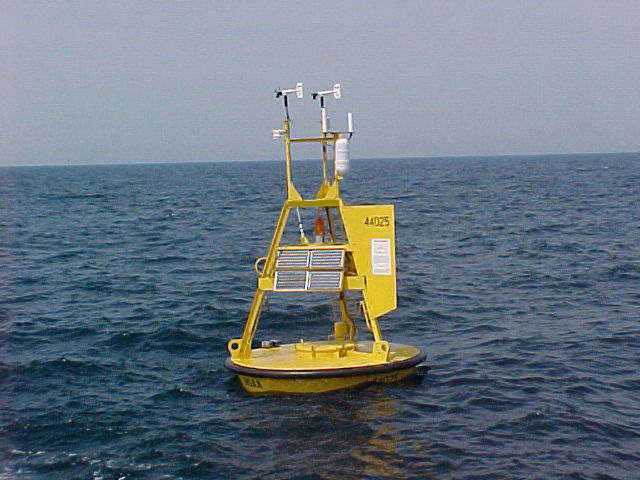
\includegraphics[height=6cm]{Figures/Chapter4/NDBCbuoy.jpg} }}%
    \qquad
    \subfloat[\centering CDIP Datawell Waverider Buoy ]{{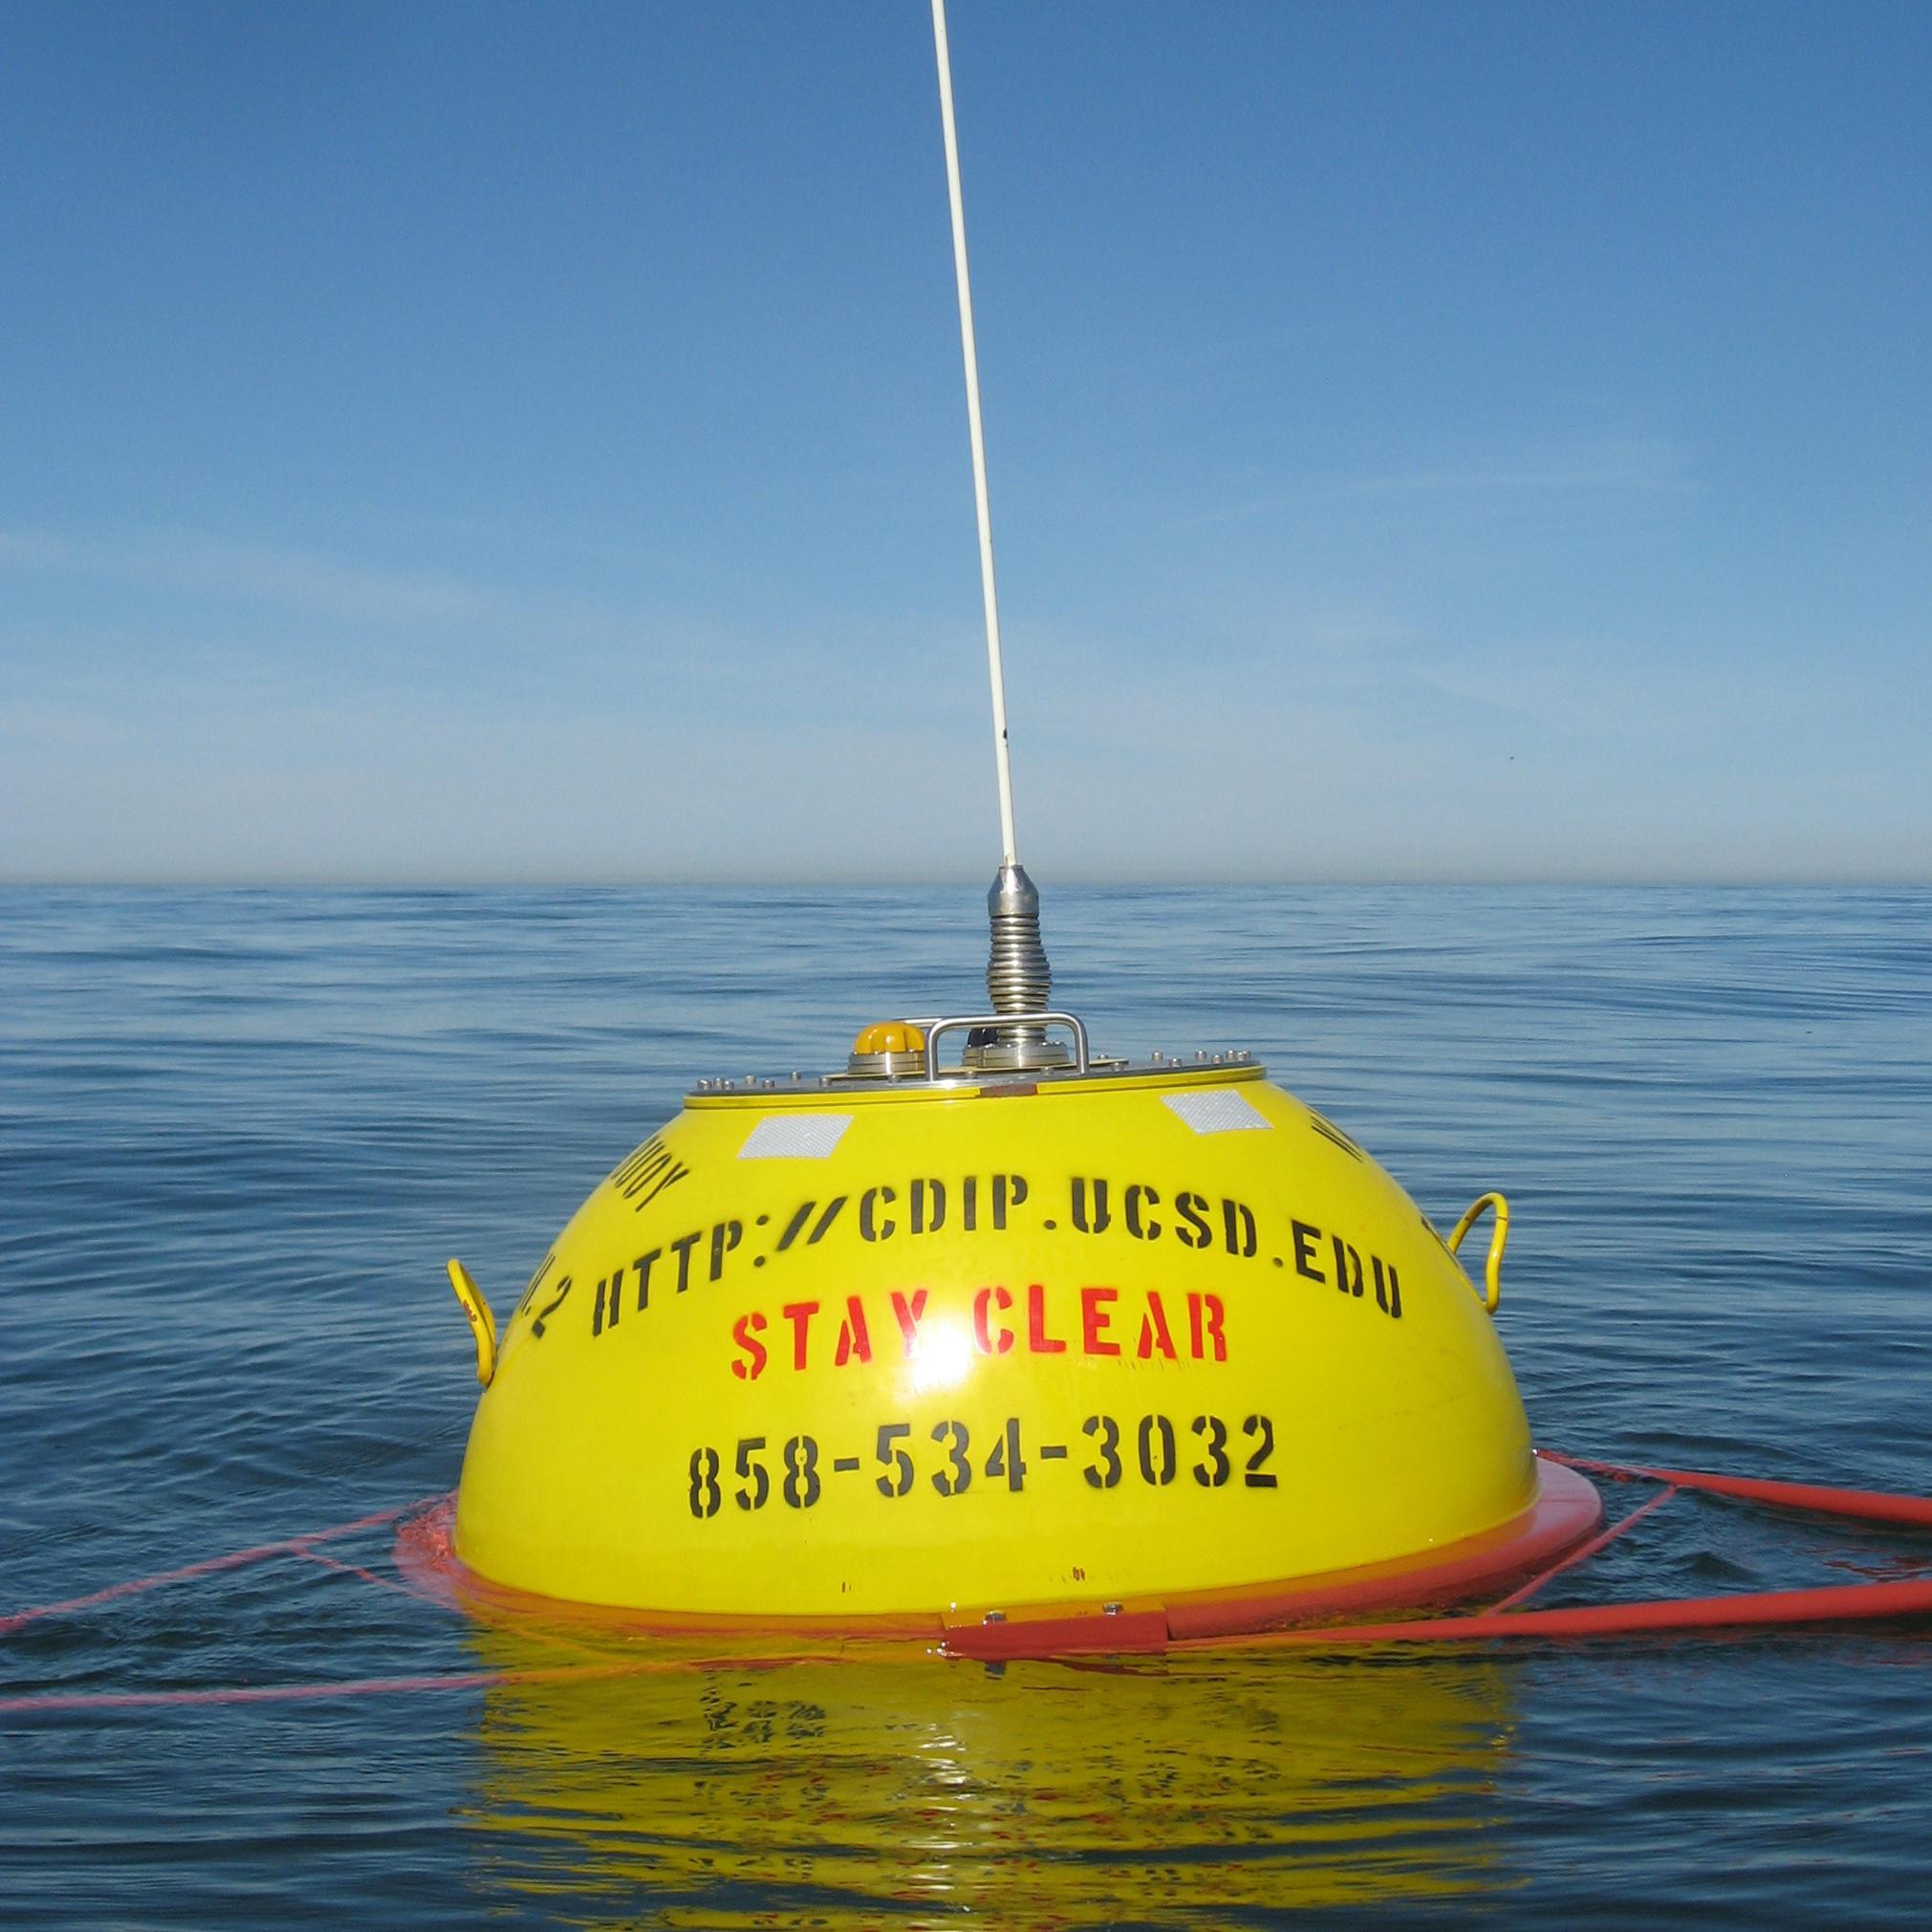
\includegraphics[height=6cm]{Figures/Chapter4/cdip.jpeg} }}%
    \caption{The two types of buoy stations moored in SNE.}
    \label{fig:example}%
\end{figure}


Information about all stations’ location characteristics and their data availability are included in Tables \ref{buoys_location} and \ref{buoys_data_availability} respectively. The anemometer height is 4.1 meters for all buoys with available wind measurements except buoys 44020 (3.8 meters) and 44039 (3.5 meters). When is needed, wind speed is adjusted at 10 meters height, assuming neutral stability of the atmospheric boundary layer, as described in \ref{WindProfile}. 


Data are available at the NDBC and CDIP websites. Directional wave spectra for buoy 44097 were downloaded from CDIP archive at THREDDS Data Server (TDS) in NetCDF format. All other geophysical parameters were downloaded from the NDBC website as \emph{.txt} files. NDBC provides an extensive description of the measurement process, the statistical analysis and quality control of the raw data, and the various error sources in \cite{Data2009}. The buoy anemometers' reported accuracy is $\pm 1m/s$ with a resolution of $0.1 m/s$. The corresponding accuracy of the SWH measurements is $\pm 0.2 m$ with a $0.1 m$ resolution. After careful examination of the quality-controlled time series, additional filtering criteria were implemented to eliminate erroneous data.


\begin{table}[H]
\begin{tabular*}{\textwidth}{c@{\hskip 0.25in}ccccc @{\extracolsep{\fill}} ccccc}
%\begin{tabular*}{\textwidth}{c @{\extracolsep{\fill}} ccccc}
\toprule
 Buoy \# &                    Location &  Lon. (deg. W) &  Lat. (deg. N) &  
 Water Depth (m) \\
\midrule
  44097 &           Block Island, RI  &    -71.127 &    40.969 &        48.16 \\
  44020 &             Nantucket Sound &    -70.279 &    41.493 &        14.30 \\
  44025 &                 Long Island &    -73.164 &    40.251 &        36.30 \\
  44017 &               Montauk Point &    -72.049 &    40.693 &        48.00 \\
  44065 &    New York Harbor Entrance &    -73.703 &    40.369 &        25.00 \\
  44039 &   Central Long Island Sound &    -72.655 &    41.138 &        27.00 \\
  44008 &      Southeast of Nantucket &    -69.248 &    40.504 &        74.70 \\
  44066 &      East of Long Beach, NJ &    -72.644 &    39.618 &        78.00 \\
  44091 &                Barnegat, NJ &    -73.769 &    39.778 &        25.60 \\
  \bottomrule
\end{tabular*}
\caption {Buoys' location, coordinates and water depth.}
\label{buoys_location}
\end{table}


 Specifically, WS data with values smaller than or equal to 0.2 m/s and SWH values lower than or equal to 0.1 meters were discarded. Previous studies \cite{Andreas2012} have used even stricter filtering criteria for the WS, recognizing that one disadvantage of the 4-blade, wind-vane sensors onboard buoys, is that they need a minimum, nonzero WS to start measuring and recording data reliably. The 0.1 meter-limit for SWH is also used by CDIP. Furthermore, data availability in terms of years of available data, as documented in Section~\ref{buoys_data_availability}, imposes the need for consistency on the final buoy time series. The final buoy datasets consist of data from 2007 until the end of 2019. Buoy time series have gaps owing to maintenance or change of the sensor payloads. The main goal was to have at least ten years of data for each buoy for consistent analysis. Previous studies have also documented that ten years of wave data are enough to characterize the seasonal variability for a specific location \cite{athanas1995}.
 
 For this reason, buoy 44091 data were used only for the validation with altimeter data. Buoy 44039 data has two disadvantages that prevented their use for other than the validation with altimeters section of this study. 


\begin{table}[H]
\centering
\begin{tabular*}{0.85\textwidth}{c@{\hskip 0.25in}cccc @{\extracolsep{\fill}} cccc}
%\begin{tabular*}{\textwidth}{c @{\extracolsep{\fill}} ccccc}
\toprule
 Buoy \# &  Distance to Coast (km)  &  Data Type & Data Availability (Years) \\
\midrule
  44097 &            41.0 &  wave only &        2009-Present \\
  44020 &            13.0 &  wind/wave &        2009-Present \\
  44025 &            42.0 &  wind/wave &        1975-Present \\
  44017 &            30.0 &  wind/wave &        2002-Present \\
  44065 &            23.0 &  wind/wave &        2008-Present \\
  44039 &            13.0 &  wind/wave &           2004-2019 \\
  44008 &           103.0 &  wind/wave &        1982-Present \\
  44066 &           121.0 &  wind/wave &        2009-Present \\
  44091 &            27.5 &  wave only &        2014-Present \\
  \bottomrule
\end{tabular*}
\caption {Buoys' distance to the closest coast and data availability depending on the type of the reported parameters and its period.}
\label{buoys_data_availability}
\end{table}


  Specifically, SWH values have a precision of one decimal number, and dominant periods are rounded to the closest integer. Data are also recorded at irregular times, which creates challenges for interpreting the results, especially compared to the other buoys' stable recording times.



\begin{figure}[H]
\centering
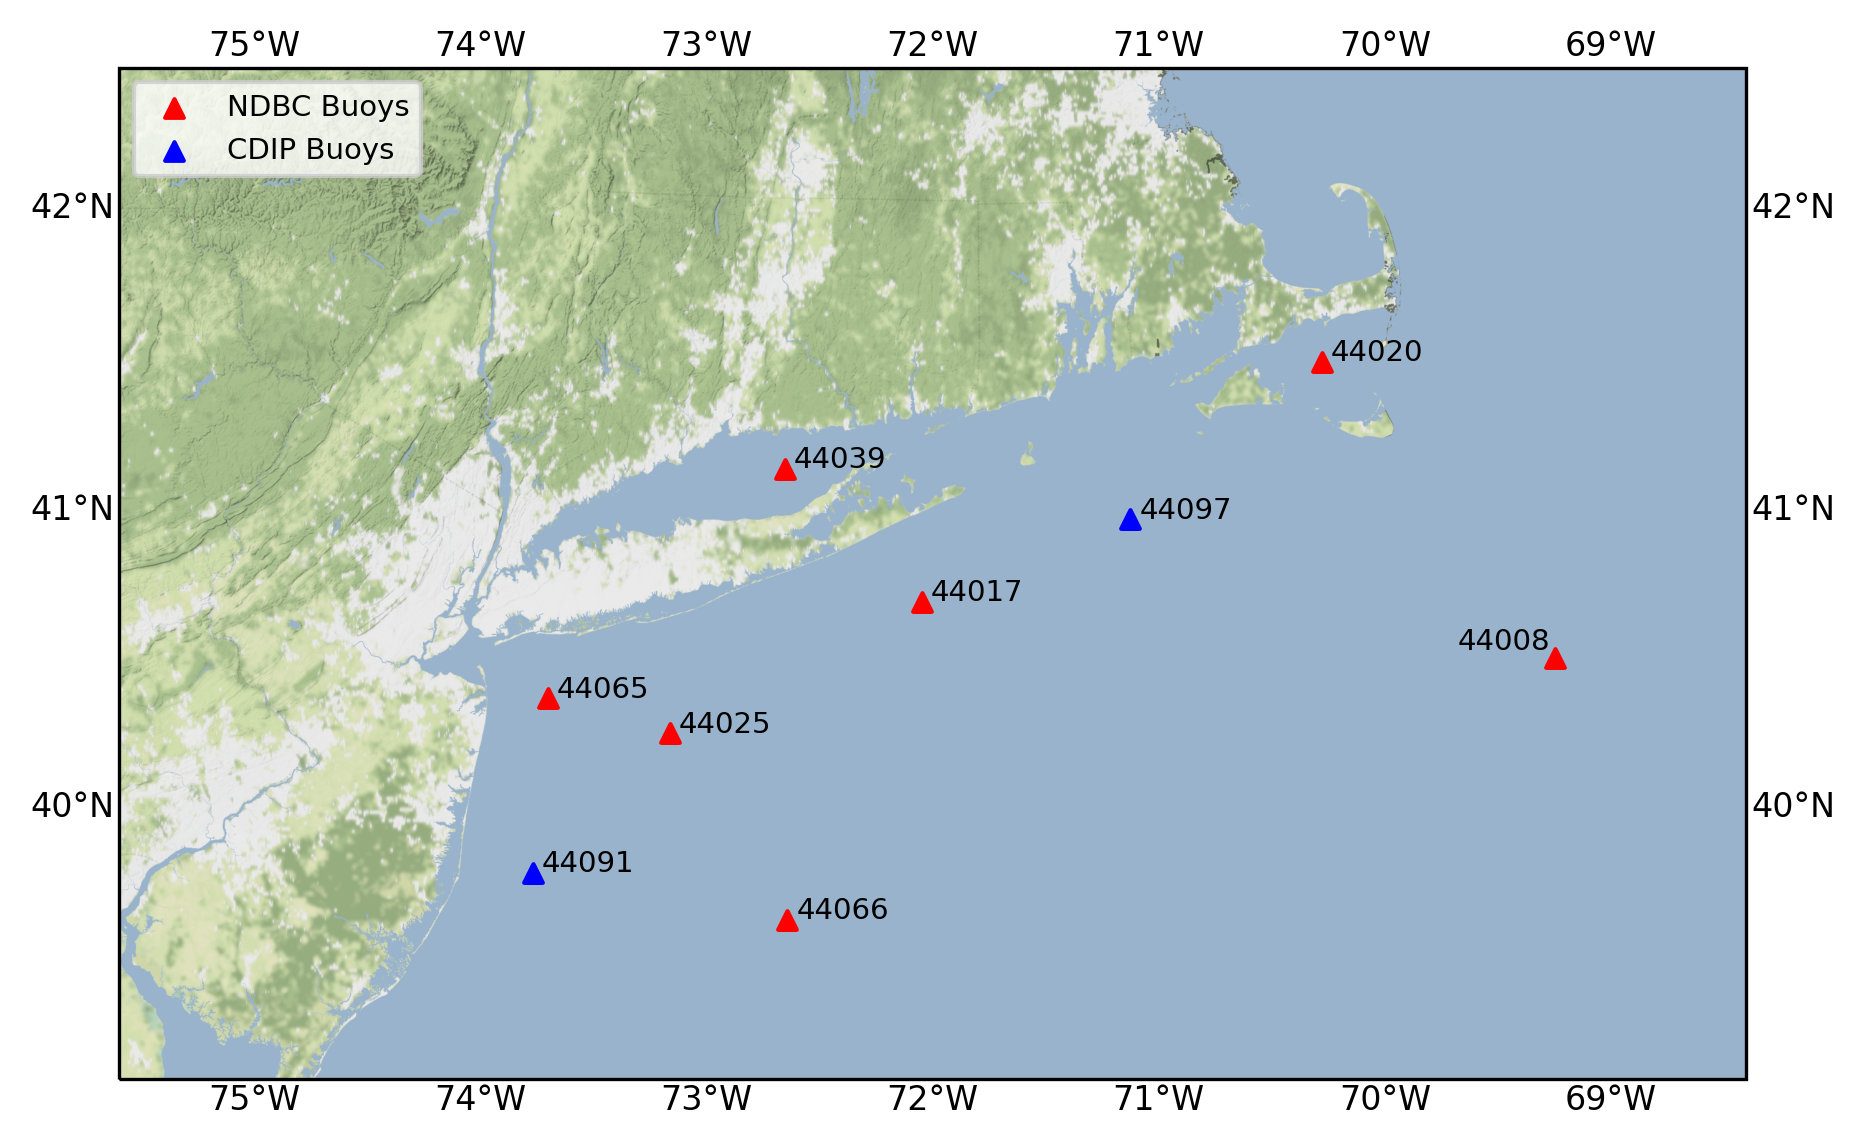
\includegraphics[width=0.95\linewidth]{Figures/Chapter4/ndbc_cdip2.png}
%\decoRule
\caption{NDBC and CDIP buoys in the SNE region.}
\label{fig:buoys_SNE}
\end{figure}


It is essential to mention the different datasets that were used and their unique characteristics. First of all, buoy payloads can record WS and wind direction in two distinct ways described in \cite{Data2009}. The first one is an 8-minute average of 1Hz observations, which leads to an hourly dataset. Data are reported at the end-of-acquisition minute, but that does not mean that the observation value includes measurements from the whole hour. This dataset was used when synchronous wind and wave observations were needed to validate altimeter data. The second one is a 10-minute average of the 1Hz observations, which is reported again at the end-of-acquisition minute. Still, the difference is that it is the average of the whole 10-minute period. This dataset is referenced as the 10-minute average dataset from now on, and it is especially useful for studying the diurnal variability and wind climate. It is also the recommended dataset for wind observations, according to BOEM for offshore wind-related studies \cite{DNVGL2018}. The 10-minute average dataset is used when wind data are processed independently, and the hourly dataset is used when combined with wave data.



Wave data are measured and reported in an entirely different way due to their more complex nature. All wave parameters are derived from the estimated energy spectra \cite{Data2009}; therefore, they are neither instantaneous nor average values of continuous observations. Wave parameters represent observations every 20 minutes. The acquisition time starts at the 20th minute of each hour and ends at the 40th. The final reported measurements are synchronized to the closest hourly wind observations. This is useful when we want to study, for example, the relationships between WS and SWH. Still, at the same time, we have to consider that the observations are not simultaneous in reality.
Data organization and preprocessing were implemented using Python \emph{Pandas} and other supplemental packages of the Python programming language. The final time series were saved as separate \emph{.txt} files for each buoy and are available for future use.


%---------------------------------------------------------------------------------------------


\subsection{Altimeter Data Collection and Organization}\label{altimeter_data}


The theoretical aspect and the distinct qualities of the satellite altimeter observations are already emphasized in \ref{AltimetryPrinciples}. This chapter will provide the necessary information regarding the altimeter datasets' characteristics, the reasons for their choice, and their actual use as input to the analysis.



\begin{table}[H]
\begin{tabular*}{0.98\textwidth}{c@{\hskip 0.25in}ccccc @{\extracolsep{\fill}} ccccc}
%\begin{tabular*}{\textwidth}{c @{\extracolsep{\fill}} ccccc}
\toprule
         &     SARAL &                  Jason 3 &      Sentinel 3A &      Sentinel 3B &        Cryosat 2 \\
\midrule
      Repeat Cycle &               35 &                       10 &               27 &               27 &              369 \\
    Frequency Band &             Ka/C &                     Ku/C &             Ku/C &             Ku/C &             Ku/C \\
 Data Availability &  03/2013- &          09/2016- &  03/2016- &  05/2018- &  07/2010- \\
 
        Instrument &           AltiKa &              Poseidon-3B &             SRAL &             SRAL &            SIRAL \\
    Operation Mode &              LRM &                      LRM &              SAR &              SAR &    LRM/SAR \\
      Product Type &              GDR &                      GDR &              NTC &              NTC &              GOP \\
  \bottomrule
\end{tabular*}
\caption {Satellite Altimeters used in this study and their characteristics.}
\label{altimeters}
\end{table}



First of all, this study's scientific context dictates the use of data from multiple altimeter missions. Currently, there are six satellite altimeters in orbit. Information about the main characteristics of each altimeter that is included in this study is provided in \ref{altimeters}. Data from the most recent altimeter mission, the Chinese HY-2B, were not used or examined. Sentinel-3A and Sentinel-3B satellites are part of the same mission, often characterized as \enquote{twins} because they have complementary orbits. They are the only satellites equipped with multiple sensors, including the radar altimeter instrument SRAL.

Satellite with ARgos and ALtiKa (SARAL-AltiKa) is a collaboration between the Centre National d'Etudes Spatiales (CNES) and the Indian Space and Research Organization (ISRO) \cite{Verron2015} with the participation of the European Organization for the Exploitation of Meteorological Satellites (EUMETSAT). This mission is unique, mainly for two reasons. SARAL-AltiKa is the first mission that takes advantage of the high-frequency Ka-band (35.75 GHz) capabilities. Specifically, its high-frequency signal means that the altimeter footprint is smaller, leading to better spatial resolution and more accurate measurements, in particular close to the coast. The disadvantage of Ka-band's high frequency is its sensitivity to water vapor and rain, leading to signal attenuation and making the atmospheric corrections even more challenging \cite{Bonnefond2018, Tournadre2009}. SARAL-AltiKa is also unique because it was launched using the same orbit and ground tracks as its predecessor mission, ERS, from March 2013 until July 2016. From July 4, 2016, it has entered its second phase, which is called the drifting phase or SARAL-DP. Since then, SARAL-AltiKa does not maintain its altitude; therefore after each repeat cycle, its ground tracks are no longer passing from the same location as the previous, but they \enquote{drift} a few kilometers. The mission agencies made this decision to preserve a few more years of its lifetime. It has been proven that it is possible to maintain good mesoscale sampling even without keeping the same altitude for the satellite \cite{Dibarboure2018}.


The Jason 3 mission involves CNES, the National Aeronautics and Space Administration (NASA), EUMETSAT, and the National Oceanic and Atmospheric Administration (NOAA). It is the successor of Jason 2, and it was launched on January 17, 2016. Jason 3 entered its calibration and validation phase on February 19, 2016, when it also started measuring and reporting data. Its primary instrument, the Poseidon-3B altimeter, sends and receives its impulses in Low-Resolution Mode (LRM), and it operates in Ku-band (13.575 GHz). Jason 3 is also unique because it has the highest temporal resolution and the lowest spatial resolution of all the altimeters. Every repeat cycle covers ten days, and every ascending or descending along-track is at an approximately 2.8 degrees distance from the closest. The instruments onboard Jason 3, which are also common to satellites that include altimeters, are shown  Figure~\ref{fig:jason3_payload}.

Sentinel 3 mission is organized and implemented by the European Space Agency (ESA) and EUMETSAT. Satellite altimetry is one of its main objectives, but not the exclusive. Its payload also includes instruments that measure and record Sea Surface Temperature (SST) and Ocean Colour data that are equally important to the geophysical parameters derived from the radar altimeter. So far, Sentinel 3 is comprised of two satellites, Sentinel 3A and Sentinel 3B. Sentinel 3A launched on February 2016 and Sentinel 3B on April 2018. They are often characterized as the \enquote{twin mission} because their along-tracks are complimentary to increase spatial coverage. Both satellites are equipped with the same payloads; hence they will be referenced in this study as Sentinel 3. Sentinel 3 SRAL altimeter sends and receives its impulses in Ku-band. It is also worth mentioning that it is the first mission that operates in SAR (or delay-Doppler \cite{KeithRaney1998})  mode exclusively, even if it can function in both SAR and LRM modes. As a result, only the across-track resolution of its effective footprint is still pulse-limited because the along-track resolution is increased and constrained to 300 meters. Conventional altimetry operates in low-resolution mode, which is pulse-limited on both the across and the along-track directions. SRAL altimeter’s received pulses can also be processed in Pseudo-Low Rate Mode (PLRM) and produce LRM-like waveforms when operating in SAR mode. Still, PLRM's estimates are noisier and have worse performance in coastal regions \cite{Nencioli2019}. In this study, only SAR mode data are used and evaluated.

Cryosat 2 is an ESA mission launched on April 2010, and its primary objective is to monitor the Arctic sea ice extent. It is a pioneer altimeter mission because it is the first-ever to operate in SAR mode. Specifically, the SIRAL altimeter onboard Cryosat 2 can operate in three modes: LRM, SAR, and SAR Interferometry (SARIn). Generally, SIRAL operates like a traditional altimeter in LRM mode. SAR processing mode is available for a few oceanographic areas, specific for each cycle. SARin is only available for the ice sheet margins and over mountain glacier regions. Therefore, Cryosat 2 data used in this study are LRM-processed with very few exceptions that are processed using the SAR waveforms. Cryosat 2 has the most extended repeat cycle (369 days) with an approximately 30-day subcycle covering a specific region of interest. It is also worth mentioning that its orbit does not repeat after completing every cycle, unlike every other conventional altimeter mission, which makes it unique in that regard.

For each mission, there are three types of dataset files available: a reduced dataset that contains only the 1Hz data, a native or standard including both the 1Hz and the 20Hz parameters, and an expert or enhanced sensor product that includes the full waveforms. Only the native dataset was collected, organized, and used for this study. 


\begin{figure}[H]
\centering
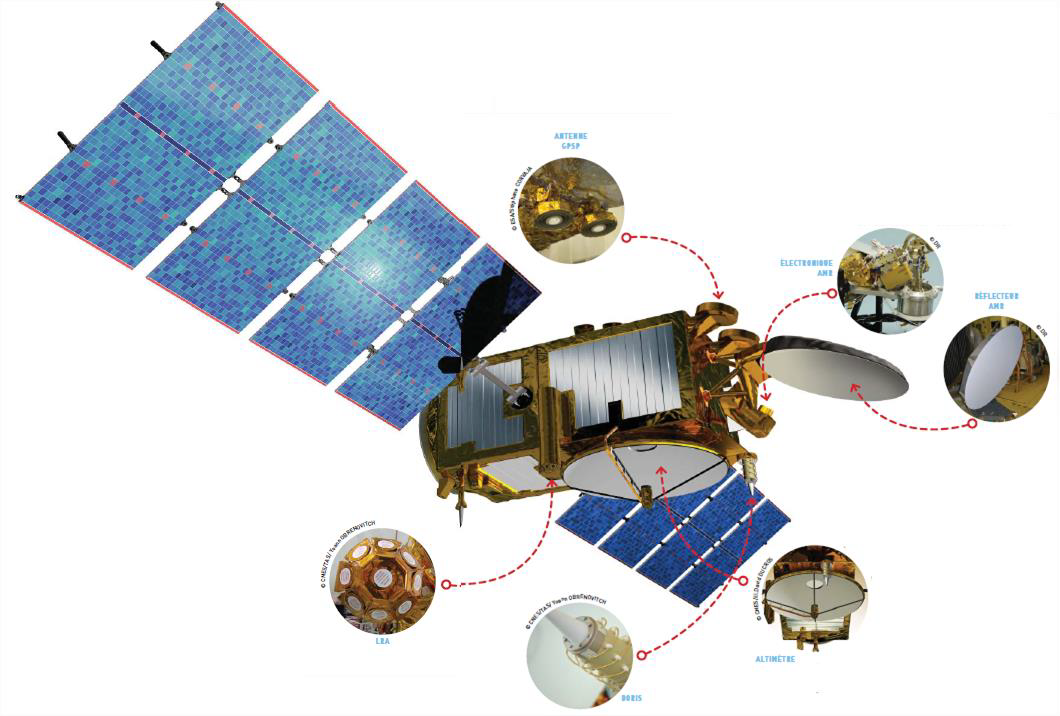
\includegraphics[width=0.95\linewidth]{Figures/Chapter4/jason3_payload.png}
%\decoRule
\caption{The main components of Jason 3 payload including the radar altimeter Poseidon-3B (center), the Advanced Microwave Radiometer (AMR, upper center) and the radio positioning DORIS system for the precise determination of its orbit (lower center). Other instruments include a Laser Reflector Array (LRA) used for the calibration of the orbit determination system (lower left) and a precision Global Positioning System Payload (GPSP) antenna (upper left). These components are common to all satellites that contain altimeter instruments. Derived from: \cite{Jason32018}}
\label{fig:jason3_payload}
\end{figure}



Besides, every altimeter mission has a family of three distinct Level 2P (processed) product types, distinguished by increasing latency and accuracy. This family of products is often called Geophysical Data Records (GDR). Near Real-Time (NRT) or Operational GDR (OGDR) products are mainly useful for the operational community. They are disseminated only a few hours after the initial waveforms are received, but they may contain outliers. Short Time Critical (STC) or Interim GDR (IGDR) products have additional auxiliary data used in the processing, and they are provided a couple of days after the NRT products. The third product type is the Non-Time Critical (NTC), or GDR, and the only one used in this study. For Cryosat 2, this product type is called Geophysical Ocean Product (GOP) to distinguish it from the ice processors’ GDR dataset. LRM products are followed by an additional M letter (GOPM) and SAR products with an R (GOPR). These products are delivered typically one month or two months after data acquisition with more precise orbit determination and atmospheric corrections. It incorporates additional auxiliary/ancillary data with lower errors.

There are different dataset standards throughout the lifetime of each altimeter. Generally, the initial standard uses the waveform retracking algorithms and geophysical/atmospheric corrections of the calibration/validation (Cal/Val) phase. Then, depending on the instrument's skills and contemporary research developments, the initial standards are updated one or two times during every altimeter's lifetime. Specifically, in this study, Jason 3 GDR-T data are used from February 2016 until September 2016. From September 2016, the GDR-D version is used. The most recent, GDR-F version of SARAL-AltiKa data is used for its first phase (March 2013 until July 2016) and also for the period from November 2019 until July 2020. For the intervening period, the previous (GDR-T) version is used because it is not disseminated yet on the AVISO \emph{ftp} server in its entirety.

Quality control is critical during the preprocessing stage. Editing criteria should be implemented on Level 2 data to filter outliers or erroneous data and keep only the valid observations before their use in the analysis. The two primary sources of the suggested editing criteria are every mission's data handbook \cite{Bronner2013, ESA2019, EUMETSAT2017, Mertz2017, Jason32018}, and the Quality Assessment Reports (QAR) that accompany the data files after the completion of each cycle. Generally, the discarded observations are not extensive due to the high data quality from the current missions. As already discussed, each altimeter has its unique features. For example, SARAL-AltiKa’s Ka-band is more sensitive to rain and water vapor. Simultaneously, it is expected to provide more observations with higher accuracy close to the coast because of its smaller wavelength and effective footprint. These characteristics are also reflected in the valid altimeter data for each mission. It is the user's responsibility to select the suitable editing criteria according to the application. For this study, we use the official mission handbooks and QAR guidelines to filter suspect or erroneous Level 2 altimeter data.

Although there are multiple sources of satellite altimetry data, SARAL-AltiKa and Jason 3 GDR data were downloaded from the \href{https://aviso-data-center.cnes.fr/}{Aviso-CNES Data Center} website, Sentinel 3 NTC data were downloaded from the \href{https://coda.eumetsat.int/#/home}{EUMETSAT Coda} website, and Cryosat 2 data were downloaded using ESA’s Cryosat User Tool (CUT).

For the preprocessing stage, NetCDF data files were input, subsetted, filtered using Python \emph{xArray} \cite{Hoyer2017} package, and the final, quality-controlled data were written to single, \emph{.txt} files using Python \emph{Pandas} \cite{McKinney2010} to be available for future use.


%----------------------------------------------------------------------------------------

\section{Spatio-temporal collocation}\label{collocation}


The satellite altimeter products consist of point observations that are representative of the nadir-pointing sensor’s footprint center. We have previously discussed that the altimeter's effective footprint cannot be considered a single point, though. It has a radius that is not constant and changes with respect to the sea state. This is also important when we want to compare altimeter measurements' accuracy against the buoys, which are stations in point locations.

A review of the different validation approaches, terminology, and metrics to assess the quality of satellite observations is available in \cite{Loew2017}. Validation is a process that requires the determination of specific criteria by the user to accomplish two primary goals. First of all, there should be limits to the two datasets' proximity both in space and time. The process of applying these limits is called spatiotemporal collocation and results in the final datasets with the collocated observations to compare. Indeed, the validation of altimeter against buoy observations is sensitive primarily to selecting the collocation or sampling radius and secondarily to the chosen time window \cite{Hwang1998}. It has been documented that a reduced sampling radius or closer proximity of the two observations in space leads to smaller absolute differences between the two collocated values \cite{Monaldo1988}. Traditionally, for global scale validation of 1 Hz altimeter data, a sampling radius of 50 or 25 kilometers and a time window of 30 or 60 minutes is selected. The data are again quality-controlled to remove possible outliers. The individual measurements are then straightforward or weighted averaged to compare with the buoy observations because they are considered simultaneous with a spatial distance of 6 to 7 kilometers \cite{Durrant2009, Queffeulou2004, Yang2019}. The selection of a suitable sampling radius becomes challenging when approaching a coastal region due to the land contamination of the waveforms and the number of available stations. The former is discussed in \ref{AltimetryPrinciples}, and the latter is the second goal we must achieve, the statistical significance of the results. Validation is often a compromise between the two, and selecting the appropriate sampling radius and time window depends on the application.


There are inherent sources of measurement error in both types of observations. The accuracy of WS and SWH measurements from buoy sensors is reported in \ref{buoy_observations}. On the other hand, the challenges of coastal altimetry are explained in \ref{AltimetryPrinciples}. The primary sources of inaccuracy in altimeter measurements include estimating parameters like the backscatter coefficient or the altimeter range from the waveform retracking and the empirical nature of the algorithms used to calculate the final geophysical parameters (SSH, SWH, WS). Hence, instrumental errors are the first source of uncertainty when comparing two different measurement systems' observations. Even if the two measurement systems had zero or identical uncertainty, their comparison would still be challenging due to their diverse spatial and temporal sampling. In other words, we need to consider how close are the observations in space and time due to the wind and wave variability in multiple spatial and temporal scales. Furthermore, we also need to take into account the sampling variability of the two types of observations. Specifically, the reported observations from buoys as described in \ref{buoy_observations} are temporal averages, whereas the 1Hz altimeter values are considered instantaneous.


This study aims to validate wind speed and significant wave height measurements from altimeters with buoys in the SNE. There are limited buoy stations in this domain, as described in \ref{buoy_observations}. At the same time, most of the stations are located closer than 50 kilometers from the coast, which is a choice of a limit for similar studies \cite{Yang2019}. In contrast, data with proximity to land are not discarded in other studies to retain a larger sample size \cite{Queffeulou2004}. Therefore, the limits selection is a compromise between accuracy and statistical significance. Specifically, a 10-kilometer sampling radius around and a time window of 30 minutes before and after each buoy observation are chosen. The time window is reduced to 15 minutes for the CDIP waverider buoys, which have a more frequent recording of data (every 30 minutes). These criteria fulfill the first goal since the closest distance to the coast is 13 kilometers for buoys 44039 and 44020; hence, we can find a considerable amount of collocated measurements from altimeters in these locations, and we avoid erroneous data due to land contamination. Still, the sample size of collocated data gets smaller as we are approaching the coast. On the other hand, the validity of altimeter observations inside semi-enclosed basins like, for example, the Long Island Sound or in areas surrounded by land and islands like the Nantucket Sound is one of this study's goals. Besides, it has been documented that the compared observations' spatial proximity plays a larger role than the temporal proximity \cite{Hwang1998, Monaldo1988}. For the reader’s convenience, we call the two buoys mentioned above as \enquote{sheltered}, the buoys which are closer than 50 kilometers from land as \enquote{coastal}, and the ones with a distance over 50 kilometers off the coast as \enquote{open ocean} buoys. The results presented in \ref{validation_SNE} are all statistically significant, and the sample size of the collocated dataset is adequate for their interpretation. We examined the option to increase the sampling radius around the open ocean buoys. Still, we decided to be consistent with the coastal and sheltered buoys and compare them using the correlation coefficient. The 30-minute time window was selected because the hourly buoy WS and SWH datasets are used for the validation and also taking into account the buoy reporting times described in \ref{buoy_observations}.


The exact, great-circle distance given the buoys and the altimeter observations coordinates were calculated using the haversine formula \ref{eqn:haversine}, where $\theta_{1}$, $\theta_{2}$ are the latitude and $\phi_{1}$, $\phi_{2}$ are the longitude coordinates of the two locations in radians. The time difference is calculated using the dates and times of the reported observations. Once the sampling radius and time window limits are applied, the collocated dataset is created. The average calculated distance is 7 kilometers. This distance is acceptable, especially when the altimeter measurement principles and the effective footprint (2-7 kilometers depending on sea state) is considered. By selecting a 10-kilometer radius, one or two collocated 1Hz altimeter observations correspond to every buoy value. In the case of two collocated altimeter observations, the first one is located north and the second south of the buoy's location. The average of the two values is calculated and then compared with a single buoy measurement. 


\begin{equation}
D(\theta,\phi) = 2 \cdot \arcsin{\left(\sqrt{\sin^{2}{\left(\frac{\theta_{2}-\theta_{1}}{2}\right)} + \cos{\theta_{1}} \cdot \cos{\theta_{2}} \cdot \sin^{2}{\left(\frac{\phi_{2}-\phi_{1}}{2}\right)}}\right)}
\label{eqn:haversine}
\end{equation}


The comparison of the two datasets was performed with Ordinary least squares linear regression. The slope and the intercept of the linear model fit are reported. Evaluation of the comparison is realized by calculating commonly used pairwise metrics \cite{Durrant2009, Yang2019} :


\begin{equation}
Bias = \frac{1}{N} \sum_{i=1}^{N} \left(A_{i}-B_{i}\right)
\label{eqn:bias}
\end{equation}

\begin{equation}
RMSE = \sqrt{\frac{1}{N} \sum_{i=1}^{N} \left(A_{i}-B_{i}\right)^2}
\label{eqn:rmse}
\end{equation}

\begin{equation}
SI = \frac{\sqrt{\frac{1}{N} \sum_{i=1}^{N} \left[ \left(A_{i}-\bar{A}\right) - \left(B_{i}-\bar{B}\right) \right]^2 }}{\bar{B}}
\label{eqn:scatter_index}
\end{equation}

\begin{equation}
R = \frac{\sum_{i=1}^{N} \left(A_{i}-\bar{A}\right) \left(B_{i}-\bar{B}\right) }{\sqrt{ \sum_{i=1}^{N}  \left(A_{i}-\bar{A}\right)^2 \left(B_{i}-\bar{B}\right)^2}}
\label{eqn:correlation}
\end{equation}

Bias is used to assessing the systematic errors or differences between the two datasets, RMSE is the Root Mean Square Error, SI is the scatter index and R is the Pearson’s Correlation Coefficient. $A_{i}$ are the altimeter values, $B_{i}$ are the buoy values,  $\bar{A}$, $\bar{B}$ represent their corresponding mean values, and  N is the collocated dataset sample size.

All calculations described above are computationally intensive due to the size of the datasets. Python library \emph{NumPy} \cite{Harris2020} and its vectorized operations helped to efficiently optimize all computations. Regression analysis was performed, and evaluation statistics were calculated using the Python libraries \emph{Scikit-learn} and \emph{SciPy}  \cite{Varoquaux2015, Virtanen2020}.


%---------------------------------------------------------------------------


\section{Variogram Modeling and Kriging Interpolation}\label{variogram_kriging}


Variogram modeling is defined by the variogram or semivariogram estimator function, which describes a variable's correlation in space. The variogram estimator is then crucial to predicting a particular variable's values at unobserved locations and obtain information on these predictions' accuracy.

The classical variogram estimator is:


\begin{equation}
\gamma(h) = \frac{1}{2N(h)} \sum^{N(h)}_{i=1} \left(z(x_{i})-z(x_{i}+h) \right)^{2}
\label{eqn:variogram_estimator}
\end{equation}

There are also other, more robust estimator functions that we can use like, for example, the Cressie \cite{Cressie1980}, the Dowd \cite{Dowd1984}, or the Genton \cite{Genton1998} estimators. This equation's parameters will be explained based on an example using satellite altimeter data on the SNE region for the winter 2019 season. The variogram estimates (blue dots) and the corresponding model (green line), which best fits the data, are presented in Figure~\ref{fig:variogram_model}.

First of all, $z(x_{i})$ is the observed value at point x and $z(x_{i}+h)$ is the observed value at a distance h from point x. This distance is called the lag interval. Lag intervals result from a process called binning, in which we classify pairs of observations in groups based on their separation distance. Figure~\ref{fig:variogram_model} shows five groups of multiples of the first lag distance of 0.4 degrees until a maximum lag distance of 2 degrees, which can be selected by the user. \emph{N(h)} is the number of observation pairs for each lag interval and is represented by the red histogram bars. With this process, all pairs of observations are given specific values of semivariances $\gamma(h)$ on the y-axis. We use the term semivariance due to the pairs of point observations. Hence, the semivariances represent variance per observation.


\begin{figure}[H]
\centering
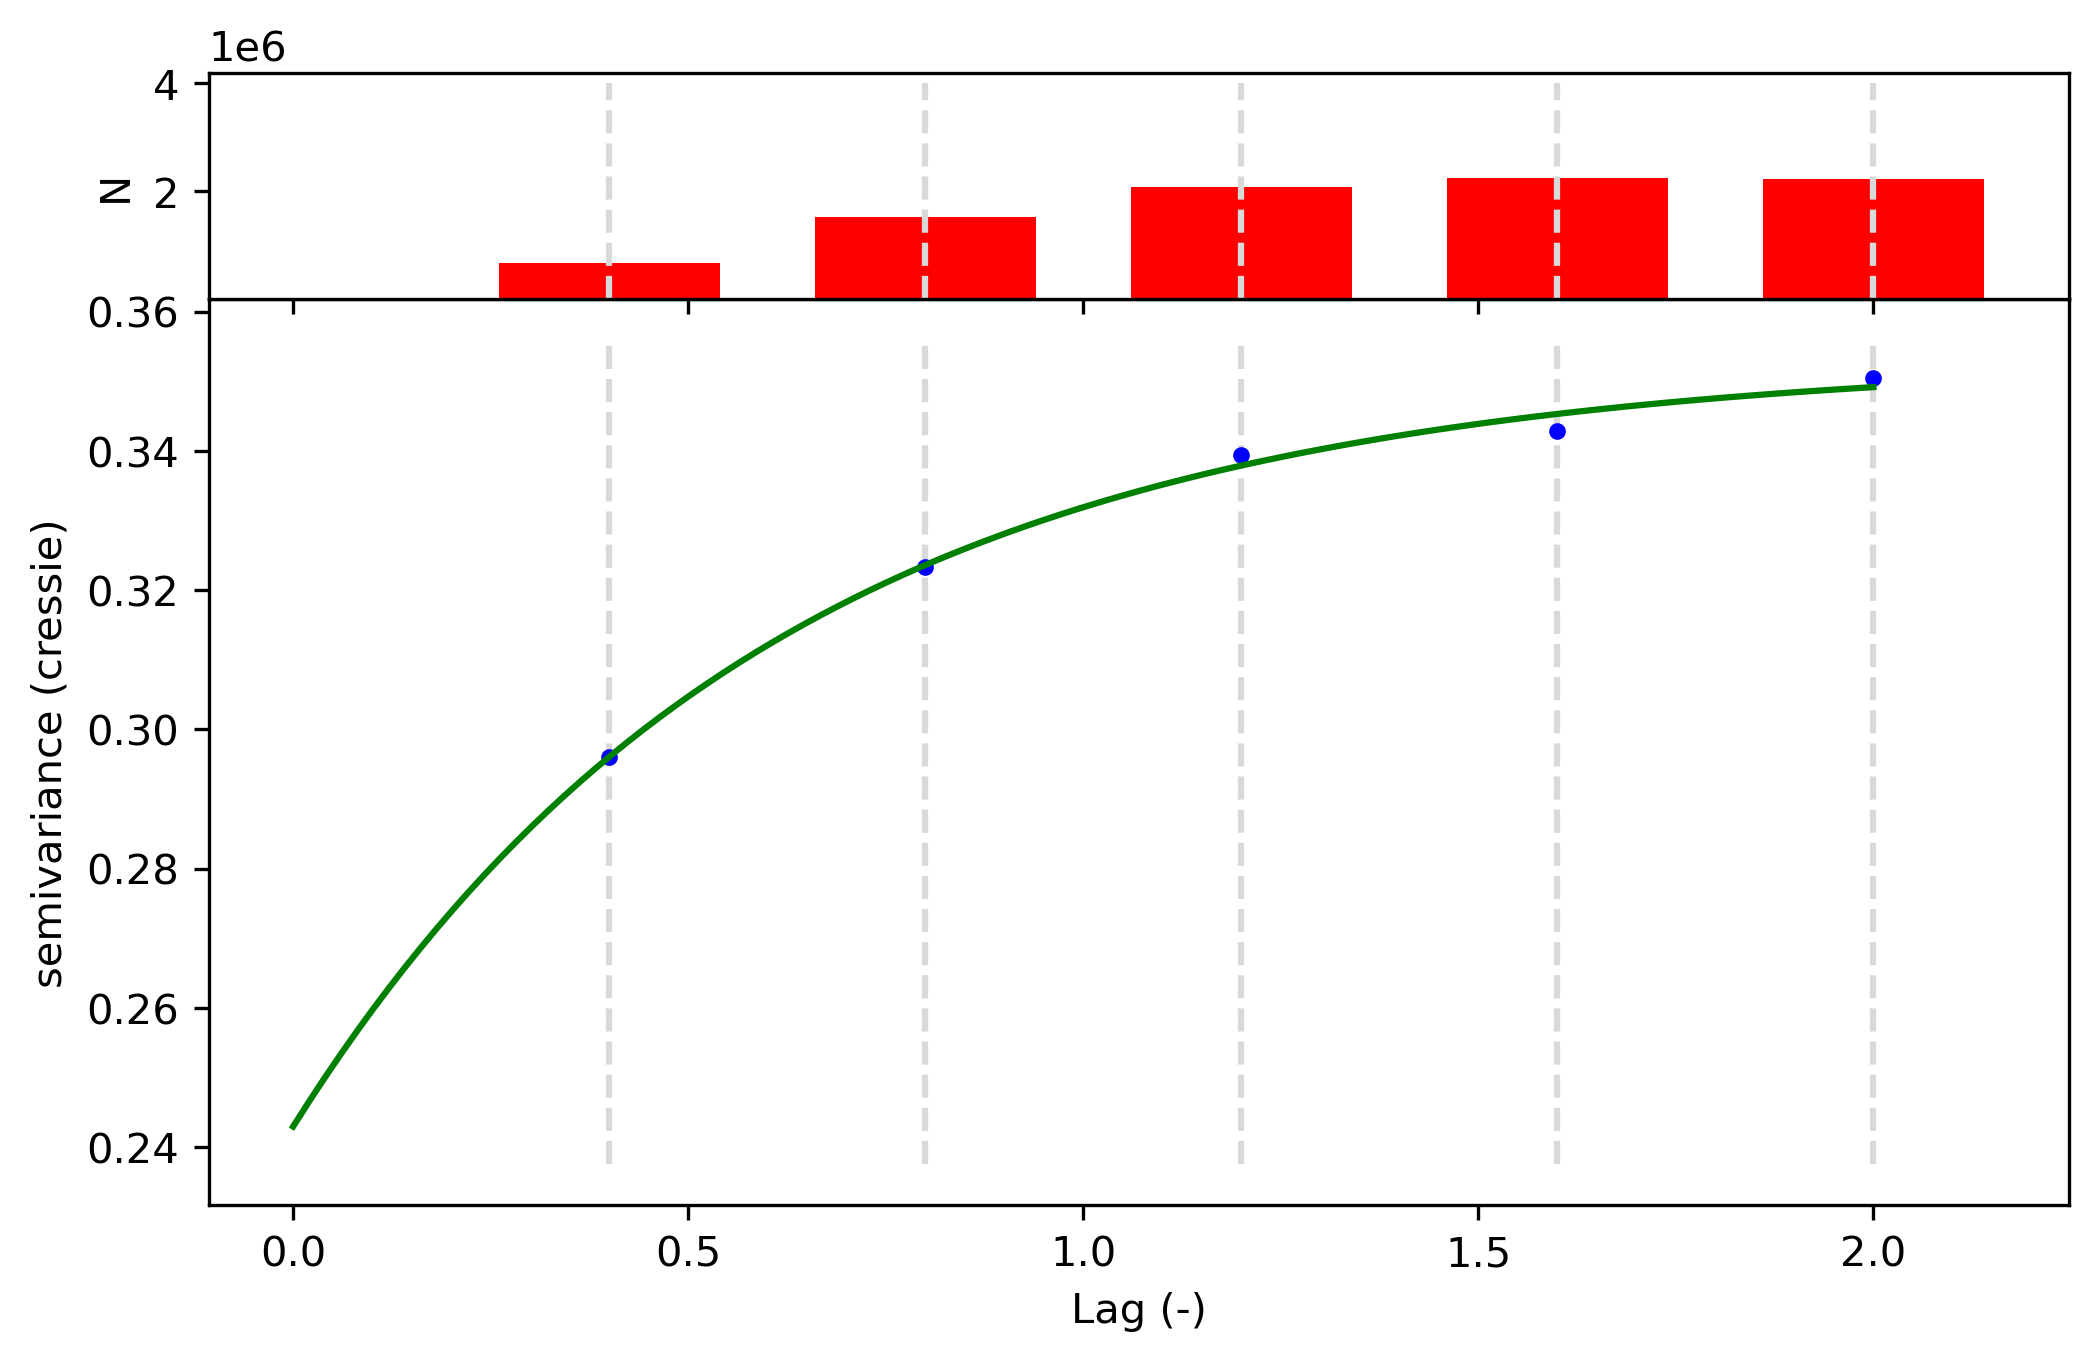
\includegraphics[width=0.8\linewidth]{Figures/Chapter4/variogram_swh2018.png}
%\decoRule
\caption{Variogram model for the satellite altimeter $H_{s}$ data for the Winter 2019 season.}
\label{fig:variogram_model}
\end{figure}


There are three fundamental parameters defined by the variogram. The first one is the sill, a variance plateau that is reached with increasing lag intervals. The sill has a value of approximately 0.11 in Figure~\ref{fig:variogram_model}. Specifically, it is called the partial sill in this example because there is an additional nugget effect, the second fundamental parameter of the variogram. The nugget can be observed as the y-intercept on the variogram (approximately 0.24 in Figure~\ref{fig:variogram_model}). It represents the minimum variance value, which exists even in zero lag interval due to small scale variations that are not captured by the large lag intervals \cite{Trauth2006}. When the nugget effect is present, the full sill is equal to the partial sill with the nugget's addition. The third variogram parameter is the range, defined as the lag distance at which the variogram reaches the sill or the partial sill if there is a nugget effect.  



Once the variogram estimator function is defined, we can fit the variogram model. Certain functions can only be used as variogram models. The most commonly used is the spherical model. Other models used to fit the variogram estimator function are the exponential, linear, Gaussian, and Matern models. Both Python libraries that were used in this study, \emph{PyKrige} \cite{Murphy2020} and \emph{SciKit GStat} \cite{Malicke2020}, provide multiple variogram estimators and models. The evaluation of each combination is performed with metrics like the correlation coefficient and RMSE and the variogram model visualization.

It is essential to mention that to perform kriging interpolation, we need to consider that the observations have to be Gaussian distributed before modeling the variogram. The variogram is sensitive to strong positive skewness resulting in higher semivariance values. Hence, if the data distribution has a long tail to the right, it is common to transform it into Gaussian using the Box-Cox transformation. An example is Figure~\ref{fig:boxcox_transform}A showing the distribution of the altimeter $H_{s}$ dataset for winter 2019. Figure~\ref{fig:boxcox_transform}B shows the distribution after the Box-Cox transformation.


\begin{figure}[H]
\centering
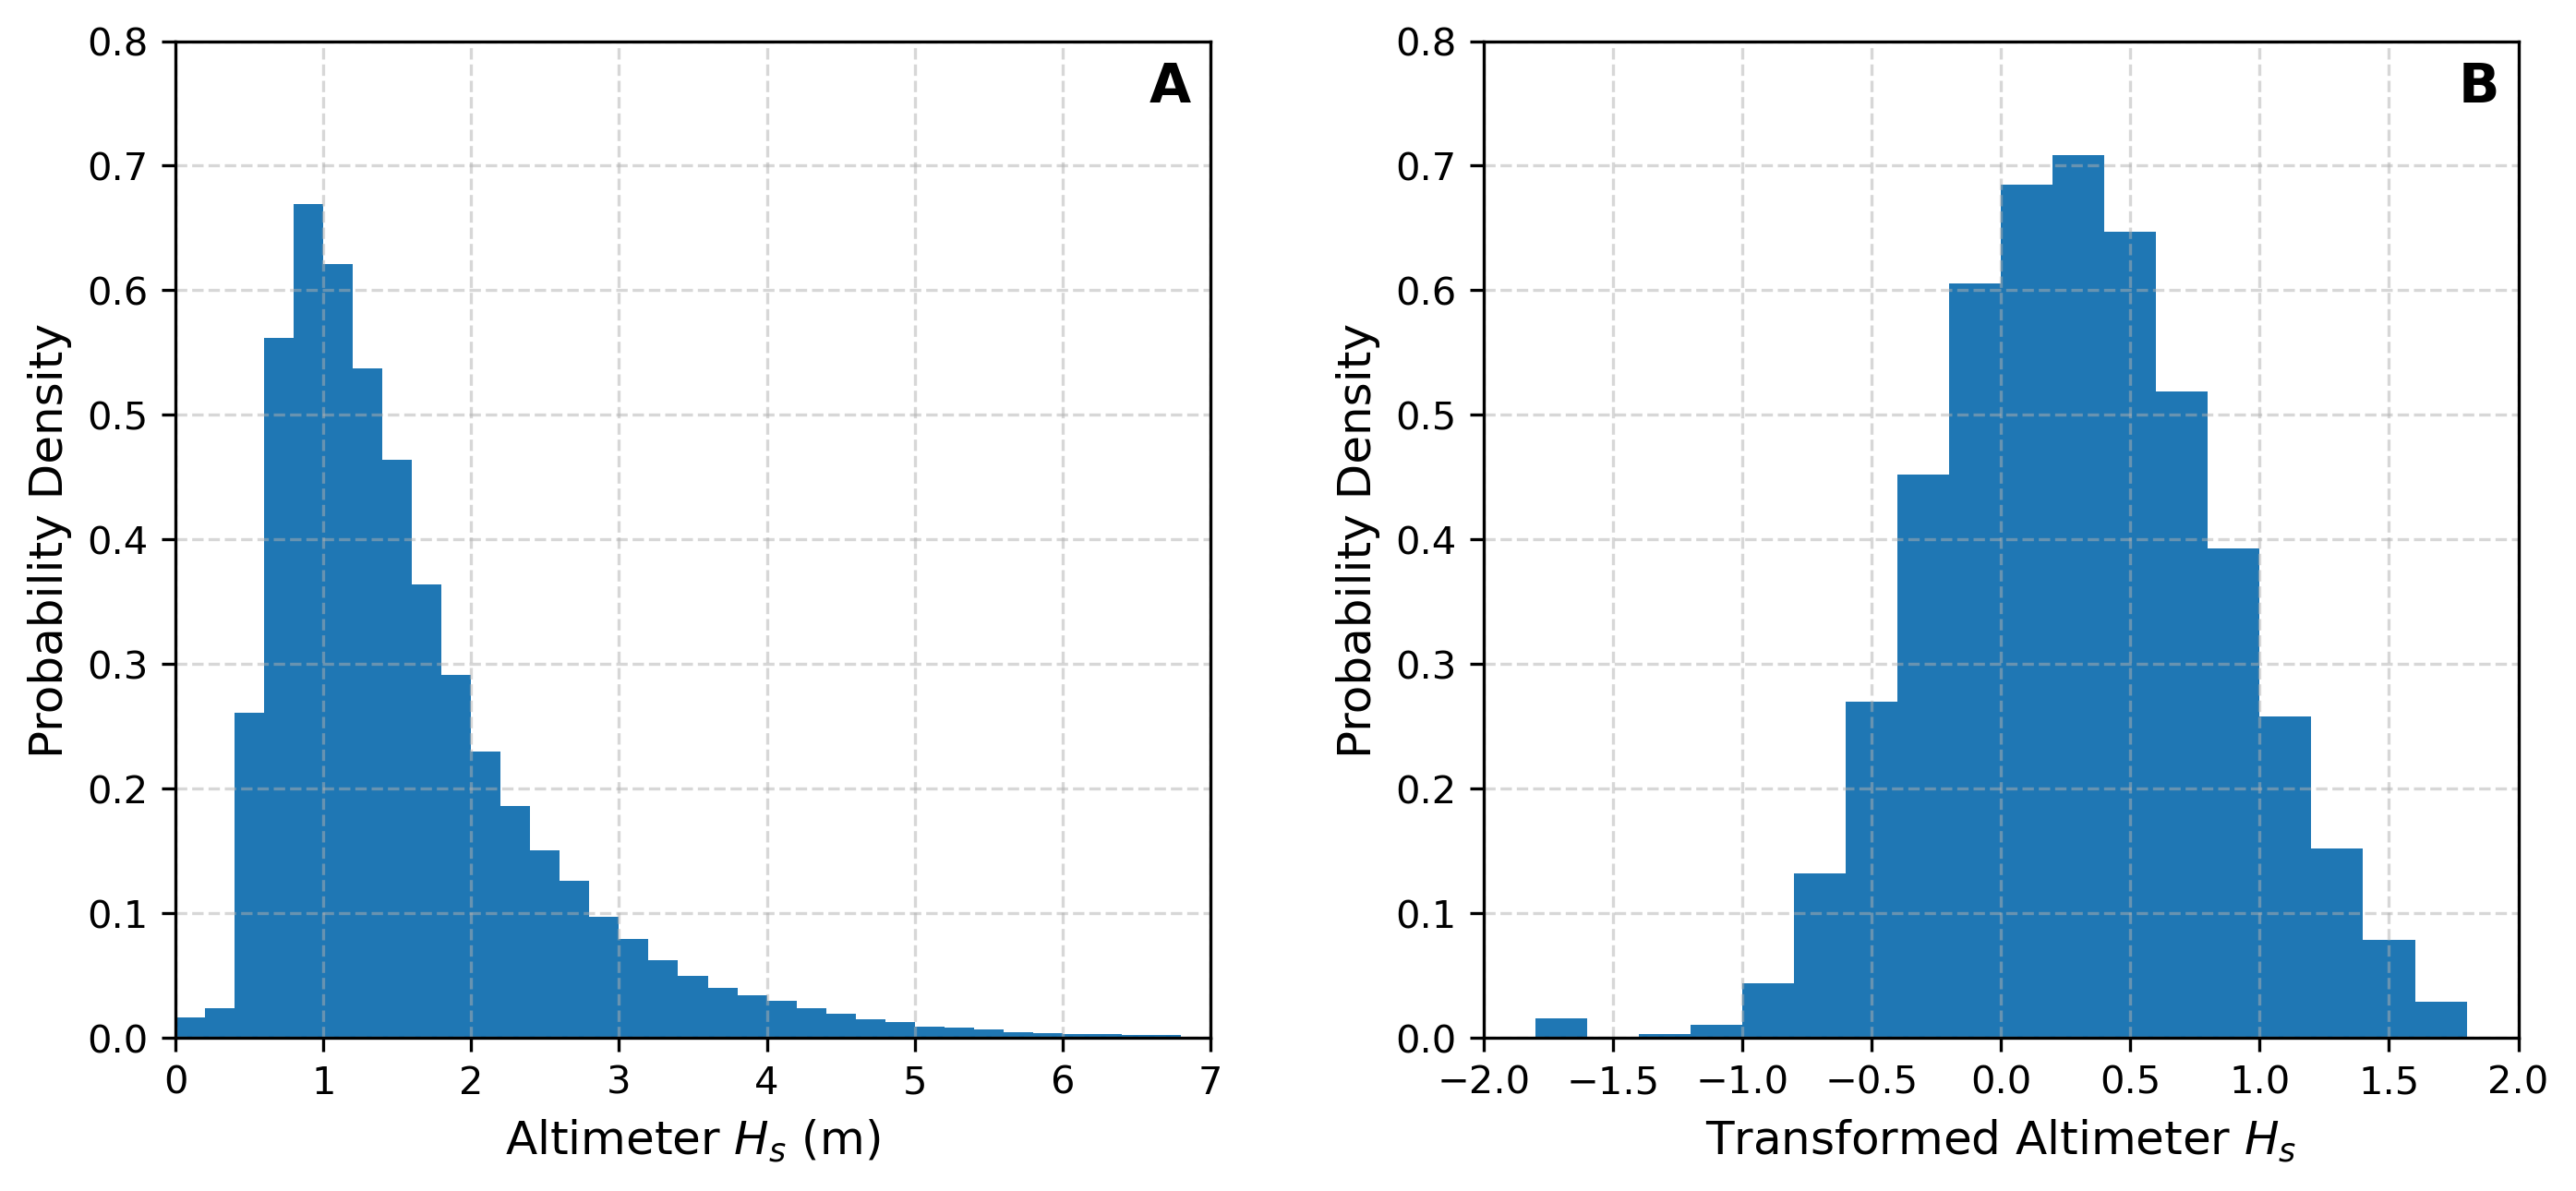
\includegraphics[width=0.85\linewidth]{Figures/Chapter4/altimeter_transobs_swh.png}
%\decoRule
\caption{A. The original altimeter $H_{s}$ distribution for the Winter 2018 season and B. The transformed to normal distribution for the same dataset.}
\label{fig:boxcox_transform}
\end{figure}



After transforming the data and modeling the variogram, we can interpolate the point observations to a regular grid. There are several types of kriging interpolation, but the most common and the one that is used herein is ordinary kriging of point observations. It is based on the assumption that we do not know the variable mean. First, the weighted average of neighboring observations is calculated to estimate a variable's value in an unobserved location.

\begin{equation}
\hat{z}(x_{0}) = \sum^{N}_{i=1} \lambda_{i} z(x_{i})
\label{eqn:kriging_interp}
\end{equation}


$\lambda_{i}$ are the kriging weights, and the condition that applies to them is that their sum should be equal to 1 to ensure that the estimates are unbiased. The value at each grid point is accompanied by a predicted error value or the kriging variance $\sigma^{2}(x_{0})$, and it is connected both with the variogram and the kriging weights.

\begin{equation}
\sigma^{2}(x_{0}) = 2 \sum^{N}_{i=1} \lambda_{i} \gamma(x_{i},x_{0}) - \sum^{N}_{i=1} \sum^{N}_{j=1} \lambda_{i} \lambda_{j} \gamma(x_{i},x_{j})
\label{eqn:kriging_error}
\end{equation}

$\gamma(x_{i},x_{j})$ is the semivariance between $x_{i}$, $x_{j}$ and $\gamma(x_{i},x_{0})$ is the semivariance between $x_{i}$ and the point we want to estimate $x_{0}$. The second condition that should be satisfied for kriging interpolation is that the estimated weights have to minimize the variances on equation~\ref{eqn:kriging_error}. This optimization is accomplished mathematically with the inclusion of Lagrange multipliers. After the solution of a system of equations, we estimate the kriging weights. Then, we estimate the variable values at the unobserved grid point locations using \ref{eqn:kriging_interp} and the kriging variance for each grid point is calculated by:


\begin{equation}
\sigma^{2}(x_{0}) = 2 \sum^{N}_{i=1} \lambda_{i} \gamma(x_{i},x_{0}) + \psi(x_{0})
\label{eqn:kriging_variance}
\end{equation}


Finally, we need to emphasize the impact of the observations' relative distance on weights. First of all, nearby point observations to the unobserved locations have higher corresponding values of weights. However, when these points are concentrated in specific areas, their weights are lower with respect to those for isolated observations. Besides, increasing nugget variance in the variogram means that the weights of nearby points become smaller.


%----------------------------------------------------------------------------------------


% Chapter 4

\chapter{Methodology} % Main chapter title

\label{Chapter4} % For referencing the chapter elsewhere, use \ref{Chapter4}

%----------------------------------------------------------------------------------------

\section{Data Processing}

\subsection{Data collection and organization}

\subsection{In situ and remote sensing data}



\cite{Stammer2017}

%----------------------------------------------------------------------------------------

\section{Spatio-temporal collocation}


%----------------------------------------------------------------------------------------


% Chapter 6

\chapter{Concluding Remarks and Discussion} % Main chapter title

\label{Chapter6} % For referencing the chapter elsewhere, use \ref{Chapter6}


Observations are essential to define the wind and wave conditions through all phases of an offshore wind farm, from the design and planning to decommission. They also enhance the quality of the numerical models' initial conditions estimation. In this study, data from buoys and satellite altimeters in the SNE region were used and analyzed.

First, we specified the normal conditions in different scales of variability using the buoy measurements due to their continuous, long-term, and reliable datasets. During the summer season, the surface WS diurnal range can reach up to 2m/s in stations with a distance of 40 kilometers or less from the closest coast. These values are lower than the diurnal range on a meteorological station on land, and the uncertainty is generally higher. The WS diurnal variability also has unique characteristics over the ocean. WS minimum values are identified six hours after the lowest WS on land and the maximum values three to six hours later. The wind direction diurnal cycle has similar patterns for the on land and offshore stations, with a lower diurnal range during the summer season for the coastal buoys. All the above do not apply for stations located over 100 kilometers off the coast, where the diurnal variability is insignificant.

SNE, a mid-latitude North Atlantic coastal region, is characterized by substantial WS and SWH seasonal variability. On the one hand, it ranges from 2m/s for the locations close to the coast to almost 4.5 m/s for the open ocean buoys. The SWH seasonal variability is negligible in areas with proximity to land and a low presence of swell waves. In contrast, it increases with distance to the coast, and it reaches up to 1.5 meters for the open ocean buoys. This difference is only partly explained by the direct influence of the wind on the sea surface. Wind roses sufficiently visualize the directional wind distribution. Generally, the wind has a west or northwest direction during the winter, while it comes from the west or southwest during the summer months. Directional wave distribution does not show the same homogeneity, especially during the winter months when higher wind speeds, storms, and swells with higher energy density are present. The directional wave spectrum of buoy 44097, located on the eastern side of SNE, reveals that the highest monthly average energy density is attributed to waves that arrive from remote regions in the Atlantic Ocean. We can also identify three systems developing throughout the year. The southeastern swell, which has energy density peaks in November and March, is the most dominant. The results indicate the importance of the directional wave spectrum for studying and monitoring the wave conditions in the SNE. Directional spectra observations can also be derived from SAR and satellite missions focused on wind and waves (CFOSAT) and assimilated into numerical models to correct their initial conditions. Therefore, the reconstruction of the directional spectrum of waves from wave buoys or NDBC stations, when available, can serve as a ground truth reference for future studies involving remote sensing observations and the evaluation of numerical models.

The relatively small number of available years of data for most buoys and the gaps in their time-series record were limiting factors for detecting statistically significant WS and SWH trends in SNE. Studies on general or extreme WS and SWH trends using in situ, remote sensing observations, and data from models show inconsistent or inconclusive results \cite{Vose2014} for the Eastern US coasts. On the other hand, the increased storm frequency and intensity in coastal regions like SNE indicate the need for further investigation.

Extreme events are also critical for offshore wind energy yield estimation and fatigue assessment on the infrastructure. Therefore, the wind and wave conditions before, during, and after the passing of a nor’easter storm are examined as a case study.

The relationships between $u_{10}$ and $H_{s}$ are calculated with polynomial regression fitting to the buoy observations for each of the primary wind directions. The relationships can adequately represent the wind and wave conditions in areas where the wind influence prevails, like the Nantucket Sound, but they are insufficient in swell-dominated locations. For this reason, the wind-wave coupling was further examined using the inverse wave age criterion that considers the wave celerity with respect to $u_{10}$. This process results in the classification of waves based on their growth, and its advantage is the inclusion of the wind and mean wave direction. The classification shows that at the coastal buoys’ locations, especially on the western side of the SNE region, the wave conditions are influenced by the wind, notably during the winter. Still, there is also a substantial presence of swell waves, which is increased during the summer months due to the decreasing wind speed. 70\% of the observations at the sheltered buoy 44020 location consist of purely wind waves, while at the open ocean buoy 44008, the sea state is swell-dominated with 95\% mixed and swell waves during the summer. We need to emphasize that relationships and classifications have their limitations, primarily because they consider only the wave spectrum's peak. A complete way to observe the sea state is by considering the whole directional wave spectrum, if available.

The accurate estimation of the WS PDF and its parameters is crucial for the offshore wind energy assessment. Specifically, the shape and scale parameters of the distribution are included in calculating the wind power output. The Weibull distribution is the most commonly used and proposed as the best fit to the WS data in similar studies. After fitting the data from four buoys located less than 40 kilometers offshore to a collection of 90 distributions and evaluating the results visually with the probability plots and quantitatively with error statistics, we suggest that the Johnson $S_{B}$ and the Beta distributions generally have exceptional performance. Only data from the sheltered buoy 44020 fit best to the Weibull 3P. The limitation of such estimations for offshore wind is that the rotor's height is greater than or equal to 100 meters, which is substantially higher than the 10-meter buoy reference height. Future studies using data from offshore towers and lidar buoys in the domain that measure WS and direction at several heights will also expand our knowledge by comparing the results included herein. Besides, even if the distributions mentioned above fit exceptionally the data from buoys in SNE, we need to examine whether mixed distribution models proposed in similar studies \cite{Morgan2011} improve our estimations.

Satellite altimetry is also an essential source of offshore wind data due to SWH and WS observations' availability to characterize both the sea state and the surface wind regime. Validation of altimeter WS and SWH against in situ observations is required to assure the quality and determine the measurements' accuracy. Although SNE is a relatively small domain with a limited number of available stations, the agreement between the collocated altimeter and buoys dataset is confirmed. The consistency is highlighted by correlation coefficient maps showing high values (over 0.9) at each buoy location to compare using the collective altimeter dataset and an increasing trend with increasing distance from the land. The results verify the exceptional performance of SARAL-AltiKa close to the coast and its ability to provide reliable measurements in low sea states.

The accumulated dataset from all five satellite altimeters was used to interpolate the observations using the kriging methodology for the 2019 winter and summer seasons. The resulting maps show strong WS gradients during winter in SNE, and further investigation is needed to assess the sensitivity of the output maps to extreme events. SWH maps show coherency during winter and summer with the highest sea states at the southeastern part of the region and decreasing SWH with increasing proximity to the land. Although the availability of SWH and WS in locations close to the coast or areas surrounded by land is one of the advantages, the estimation is not as robust as in the open ocean due to the smaller sample size and the limitations induced by topography. The various sources of errors in the estimation are documented, emphasizing the WS diurnal or sampling bias. Monitoring of the sea state and surface wind conditions requires multiple sources of data, and combined satellite datasets are analyzed in recent studies \cite{Hasager2015}. The requirement to fill the temporal gaps of the satellite altimeter observations in future studies is addressed.
% Chapter 6

\chapter{Discussion} % Main chapter title

\label{Chapter6} % For referencing the chapter elsewhere, use \ref{Chapter6}
%% Chapter 7

\chapter{Conclusion} % Main chapter title

\label{Chapter7} % For referencing the chapter elsewhere, use \ref{Chapter7} 

%----------------------------------------------------------------------------------------
%	THESIS CONTENT - APPENDICES
%----------------------------------------------------------------------------------------

\appendix % Cue to tell LaTeX that the following "chapters" are Appendices

% Include the appendices of the thesis as separate files from the Appendices folder
% Uncomment the lines as you write the Appendices

%% Appendix A

\chapter{Frequently Asked Questions} % Main appendix title

\label{AppendixA} % For referencing this appendix elsewhere, use \ref{AppendixA}

\section{How do I change the colors of links?}

The color of links can be changed to your liking using:

{\small\verb!\hypersetup{urlcolor=red}!}, or

{\small\verb!\hypersetup{citecolor=green}!}, or

{\small\verb!\hypersetup{allcolor=blue}!}.

\noindent If you want to completely hide the links, you can use:

{\small\verb!\hypersetup{allcolors=.}!}, or even better: 

{\small\verb!\hypersetup{hidelinks}!}.

\noindent If you want to have obvious links in the PDF but not the printed text, use:

{\small\verb!\hypersetup{colorlinks=false}!}.

%\include{Appendices/AppendixB}
%\include{Appendices/AppendixC}

%----------------------------------------------------------------------------------------
%	BIBLIOGRAPHY
%----------------------------------------------------------------------------------------

\printbibliography[heading=bibintoc]

%----------------------------------------------------------------------------------------

\end{document}  
